\documentclass[a4paper, 12pt]{article}
\usepackage{setspace}
\usepackage{graphicx}
\usepackage{longtable}
\usepackage[backend=bibtex,style=numeric]{biblatex}
\usepackage{mathtools}
\addbibresource{bibliography.bib} 
\graphicspath{ {images/} }
\doublespacing

\begin{document}
\title{Using Machine Learning For DOTA2 Match Outcome Prediction}
\author{Andrius Buinovskij}
\maketitle

    \section{Dictionary}

	\par There are some more obscure terms littered throughout the text. Here is a short explanation for each one.

        \begin{itemize}
            \item A \textbf{feature} is some aspect of something. For instance, a coin may have a mass, an area, an average colour and so on. Each of those are a feature.
            \item \textbf{Classification} is the problem of identifying to which of a set of categories (sub-populations) a new observation belongs, on the basis of a training set of data containing observations (or instances) whose category membership is known.\footnote{Wikipedia.}

        \end{itemize}

    \section{Introduction}

        \par This text describes four contemporary machine learning techniques, and then shows their application in match outcome prediction in a game of Dota 2, namely, which team will win, based on players' hero selection. In other words, it is classifying team composition as preferring a radiant win, or preferring a dire win.

        \par The game in question, Defence of the Ancients (DOTA) 2, is very nuanced and has a plethora of mechanics. For the purposes of this paper however, it will suffice to say that in a game of DOTA, two teams, "Dire" and "Radiant"\footnote{Dire being evil and red, Radiant being green and good.}, five players per team, try to destroy the other team's base. At the beginning of a game, each player chooses a "hero" to play, a character within the game. Different heroes have different abilities, and some heroes synergize, whilst others cancel each other out. As of writing of this text, there are 113 different heroes, resulting in a bewildering number of possible team compositions.
        
    \newpage

    \section{Background}

        \par The machine learning techniques used are: Nearest Neighbours, Neural Networks, Support Vector Machines and Boosting. The intuition and broad strokes of each are explained below, with pointers to more information should it be desired.
        
        \subsection{Machine Learning Generalities}
        
            \par In general, the (supervised, since this is what this particular project is about) machine learning pipeline looks something like this:
            
                \begin{figure}[h]
                    \caption{General machine learning process.}
                    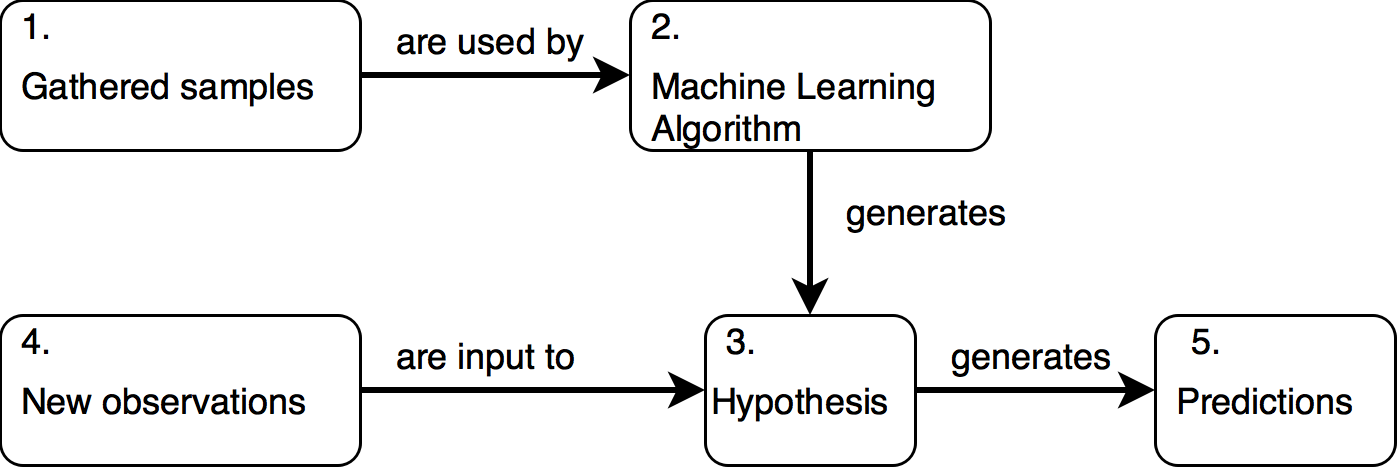
\includegraphics[width=\textwidth]{machineLearningGeneralNotion}
                \end{figure}
                
            \par We begin with some dataset of examples. This could be a list of coins, their value and their mass, or it could be a list of houses and their square footage, number of bedrooms, the price they sold for and so forth. The dataset will be split into the data, and "the label", the label being the feature the algorithm will try to learn about. 
            
            \par Then we pass this dataset to the machine learning algorithm. The algorithm will "train" a model, basically adjusting parameters of the model such that the model will perform as well as possible on the dataset, which will hopefully generalize to out-of-sample performance. 
            
            \par What is meant by performance is that, in classification, each sample will belong to some category. The more of the training sample the algorithm classifies correctly, the better is it's in-sample performance. This could be, given the square footage and number of bedrooms of a house, predict whether it is worth more than 500,000 Euro. The algorithm is trained such that it will classify correctly as many training samples as possible.\footnote{Something called regularization aside. Regularization hinders in-sample performance in order to avoid over-fitting. All the details can be found at \cite{overfitting} and \cite{regularization}.}
            
            \par This trained model or hypothesis will then be able to take some new observations, perhaps a new coin or a house description, and predict the label.
            
            \par The hypothesis is formed using the training set, but is validated using a testing set. This means that the hypothesis is tested on a set of samples that it was not trained on to see how well the hypothesis will perform in the "real world", or how well it will "generalize" to out-of-training set samples.
            
            \par For a more in-depth explanation, please see\cite{machineLearningBackground}.

        \subsection{Nearest Neighbours}

            \subsubsection{Nearest Neighbours Intuition}

                \par The simple logic behind the nearest neighbours approach to machine learning is: when asked to classify a new observation, one should see if the scenario in question has occurred before within the training set, and see what was done then. If the precise scenario has not occurred, then one should find the most similar scenario on record for guidance.

                \par Let us say that we are trying to build an algorithm which will be used as a part of vending machines, namely, deciding on the value of coins that are inserted into the machine. Let us also say that the value of the coin will be decided based solely on it's mass (for simplicity), and that we have a training set of coins already weighed and labelled.

                \par A coin is inserted into the vending machine, how can we tell it's precise value? All we have to go by is the coin's mass. Currently, our training set is illustrated below.

                \begin{figure}[h]
                    \caption{A visualization of coins placed on mass axis.}
                    \centering
                    \includegraphics[width=\textwidth]{coinAxis}
                \end{figure}
                

                \par So we have three coins of mass of 2, 5 and 10 grams. Let us say a coin is inserted into the machine, of mass of 6 grams. Here it is on our graph.

                \begin{figure}[h]
                    \caption{Coin graph including mismatching coin.}
                    \centering
                    \includegraphics[width=\textwidth]{coinAxis2}
                \end{figure}

                \par We would like to decipher the value of the newly inserted coin. An immediately obvious approach is to query our training set of already known mass-value pairs of coins to find a coin that most closely resembles the new coin, and say that the two are the same. Within the graph, this is simply looking for the nearest neighbouring coin\footnote{Hence the name of the method, Nearest Neighbours.}. Here it is again on our graph.

                \begin{figure}[h]
                    \caption{The nearest neighbour to the unknown coin}
                    \centering
                    \includegraphics[width=\textwidth]{nearestNeighbour}
                \end{figure}

                \par Having found the nearest neighbour, the 20 cent coin, we conclude that the new coin must also be a 20 cent coin, perhaps with some imperfections.

                \par This short example illustrates the benefits and shortcomings of Nearest Neighbours. The method is simple and logical, and directly uses experience of the past. However, it is not extracting underlying patterns out from underneath the data, but is instead simply\footnote{Not for long.} looking to the past for similar cases.
                
            \newpage


            \subsubsection{Adding complexity and Trees}

                \par Our coin example was quite simple, using a single feature, and just three neighbour entries. A single feature gives rise to a single axis, however, we could have used more. For instance, we could have used the coin's area, which would have looked like the following:
                
                \begin{figure}[h]
                    \caption{A visualization of coins places on area and mass axes}
                    \centering
                    \includegraphics[width=\textwidth]{twoAxes}
                \end{figure}

                \par The search for a nearest neighbour is now a two-dimensional one, which we can still handle intuitively. However, as the number of features, and consequently axes, grows, the question of how does one find nearest neighbours arises.

                \par So, how does one find the nearest neighbours, and do so efficiently? Presented are three algorithms.
                
                
                \subsubsection{Brute force}
                
                    \par Let the set of exemplar coins (the 10, 20 and 50 cent coins) be \textbf{S} and the newly observed coin be \textbf{T}. 
                    
                    \par The brute force approach to finding k number of nearest neighbours is to simply calculate the distance\footnote{The function to calculate distance preferably being a non-negative, symmetric and satisfying the triangle inequality function.} between \textbf{T} and every member of \textbf{S}, and keep the k nearest neighbours.
                    
                    \par Unfortunately, this method has a running time of \textit{O(ckn)}\footnote{or, less a less naive cn}, where c is the cost of calculating the distance function, k is the number of nearest neighbours desired and n is the number of exemplars in the set \textbf{S}.
                    
                \subsubsection{Kd-trees}
                
                    \par The idea behind kd-trees is to build a tree structure to segment the set \textbf{S} such that to find the nearest neighbours, one only has to examine one of those segments\footnote{Not quite, more on that later}. This is similar to how a human would look for a nearest neighbour on a graph. Instead of checking every point, no matter how far away on the graph, we would focus our attention on the nearby points, since the far away points are irrelevant.
                    
                    \newpage
                    
                    \par Here is a new set of exemplars \textbf{S}, to better demonstrate the algorithm.
                    
                    \begin{center}
                        \begin{tabular}{| l | l | l | l |}
                            \hline
                            Id & Feature A & Feature B & Feature C \\ \hline
                            0 & 2 & 8 & 4 \\ \hline
                            1 & 1 & 4 & 3 \\ \hline
                            2 & 3 & 5 & 7 \\ \hline
                            3 & 10 & 2 & 3 \\ \hline
                            4 & 2 & 12 & 1 \\ \hline
                            5 & 7 & 4 & 8 \\ \hline
                            6 & 5 & 4 & 9 \\ \hline
                            7 & 2 & 7 & 1 \\ \hline
                             
                        \end{tabular}  
                    \end{center}                
                    
                    \par Each row corresponds to a single exemplar, where the exemplars have three features each, namely A, B, and C.
                    
                    \par Now we are going to split \textbf{S} in two. A question arises of how to best do this. The answer is to pick the feature with the largest variance, and then choose the median value from the current set of exemplars being split.\cite{kNearestNeighbours}\footnote{The reasoning is explained under "The Optimized k-d Tree", page 7.}
                    
                    \newpage
                    
                    \par On the first pass through, the feature with the greatest variance is B. Now we choose the median value, which in this case is 4.5 (4+5/2, even numbers). So now all exemplars which have a value of B which is less than or equal to this median go to the left branch, whilst all greater than 4.5 go to the right branch, as follows:
                    
                    \begin{figure}[h]
                        \caption{A visualization of the first segmentation.}
                        \centering
                        \includegraphics[width=\textwidth]{kdTreeFirstDivision}
                    \end{figure}
                    
                    \newpage
                    
                    \par Now we do this again on both children nodes of the root. On the left-hand node, the feature with the greatest variance is A, and the median is 6. On the right-hand node, the feature with the greatest variance is B, and the median is 7.5. This is the result:
                    
                    \begin{figure}[h]
                        \caption{A visualization of the second segmentation.}
                        \centering
                        \includegraphics[width=\textwidth]{kdTreeSecondDivision}
                    \end{figure}
                    
                    \newpage
                    
                    \par Now the tree is 2 levels deep. The number of levels, and consequently the number of sections the exemplar set \textbf{S} is subdivided into is up to the person running the algorithm.
                  
                    \par That concludes the construction of the tree. Say now we have observed a new exemplar, with values A: 3, B:7, C:5. To find the nearest neighbour, we simply traverse down the tree structure. At the root, our B is 7, which is more than 4.5, and so we take the right branch. Now again we decide on B, but B is less than or equal to 7.5, so we take the left branch. From there we manually calculate distance to each of the exemplars (2 and 7) and take the closer one. We only needed to compute the distance 2 times, instead of 7 for all of the nodes.
                  
                    \par Note however that this means of finding the nearest neighbour is approximate, and is not guaranteed to find the true nearest neighbour. For that, please see the "bounds-overlap-ball" and "ball-within-bounds" functions in \cite{kNearestNeighbours}.
                    
                \subsubsection{Balltree}
                
                    \par There are many versions of the balltree algorithms\cite{manyBalltrees}, however, here we will describe the most basic version for the sake of illuminating the concept.
                    
                    \newpage
                    
                    \par The idea behind balltrees is quite similar to kd-trees, in that we are still essentially building a tree structure to segment the exemplars such that not all of them have to be examined when looking for a nearest neighbour. However, the method in which we segment the exemplars is centred around subdividing them with hyperspheres. 
                    
                    \par Suppose a balltree is to be built from the following exemplars:
                    
                    \begin{figure}[h]
                        \caption{The root of the balltree.}
                        \centering
                        \includegraphics[width=\textwidth]{balltree0}
                    \end{figure}
                    
                    \newpage
                    
                    \par Currently we have one node, the entire exemplar set. To divide it, we calculate the centroid of the current node, which looks like:
                    
                    \begin{figure}[h]
                        \caption{The root of the balltree, with centroid in red.}
                        \centering
                        \includegraphics[width=\textwidth]{balltree1}
                    \end{figure}
                    
                    \newpage
                    
                    \par Now we pick the point the furthest away from the centroid, call this \textit{p1}. Then pick a point farthest away from \textit{p1}, and call it \textit{p2}.
                    
                    \begin{figure}[h]
                        \caption{The root of the balltree, with centroid in red, p1 in green and p2 in purple.}
                        \centering
                        \includegraphics[width=\textwidth]{balltree2}
                    \end{figure}
                    
                    \newpage
                    
                    Now we calculate the distance of each point to p1 and p2. Points closer to p1 become one subset, and points closer to p2 become the other subset:
                    
                    \begin{figure}[h]
                        \caption{Two new segments of the set.}
                        \centering
                        \includegraphics[width=\textwidth]{balltree3}
                    \end{figure}
                    
                    \par Note that the circles can intersect, but each of the exemplars belongs only to one of the two new segmentations. This is done again and again until the desired granularity is achieved. 
                    
                    \par So how does one query a balltree structure? There are multiple ways, some more efficient than others\cite{manyBalltrees}, but at the core we are still simply segmenting the tree and then only looking at the relevant, close-by segments, or in this case, relevant hyperspheres. The hyperspheres and thus all the points assigned to them are decided to be relevant via some distance guarantees\footnote{which are only possible if a proper metric is used.}, the derivation for which can be found at \cite{manyBalltrees}.
                        
                \newpage
                
                \subsection{Neural Network}
                
                    \par There are two parts to neural networks, namely the individual neurons, and how they are connected to form a network.
                    
                    \subsubsection{The Neuron}
                    
                        \par The basic idea behind a neuron is: a neuron receives a set of input signals, and if the sum of those input signals is greater than the threshold, then the neuron "fires" and outputs True, "1", or some indication of excitation. Visually it looks like:
                        
                        \begin{figure}[h]
                            \caption{A simple neuron.}
                            \centering
                            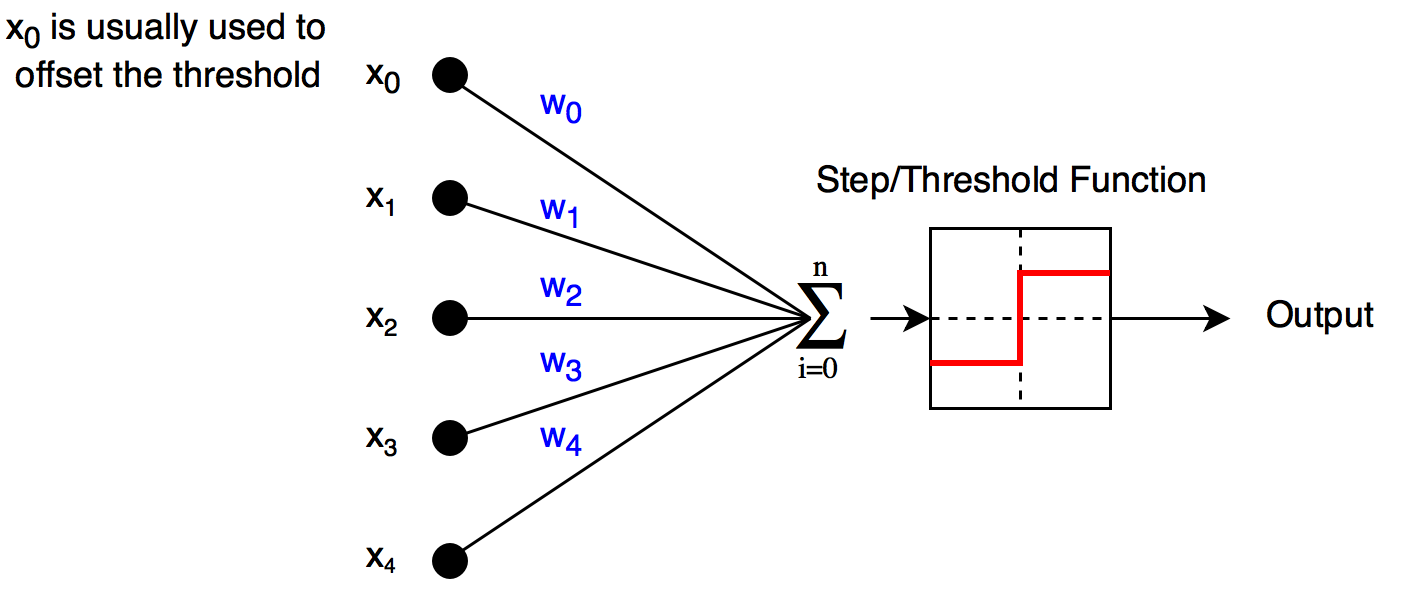
\includegraphics[width=\textwidth]{neuron}
                        \end{figure}
                    
                        \par A neuron has \textit{n} inputs, in this case, 5. Each of the inputs \textit{x\textsubscript{i}} has with it associated a weight, \textit{w\textsubscript{i}}, by which the input is multiplied. This is how different factors are emphasized/diminished, and what is adjusted during "training" of the neuron.
                        
                        \par The inputs, multiplied by their respective weights, are then summed (so x\textsubscript{0}w\textsubscript{0} + x\textsubscript{1}w\textsubscript{1} + ... x\textsubscript{4}w\textsubscript{4} in this particular example), and passed through a threshold function. In the end it looks like:
                        
                        \par \centerline{ {\large output = \(threshold(\sum\limits_{i=0}^n x\textsubscript{i}w\textsubscript{i})\) } }
                        
                        \bigskip
                        
                        \par A threshold function simply fires if the summation is more than some value. So, for example, if the threshold is 0 and if the inputs x\textsubscript{0}w\textsubscript{0} and so on sum to 0 or more, the output will be 1, and 0 otherwise.
                        
                        \par The input x\textsubscript{0} is defined as a constant 1 and the weight w\textsubscript{0} is used to adjust the threshold. If, for instance, w\textsubscript{0} is 0.5, then the entire summation of inputs is essentially shifted to the right by 0.5. If the threshold is set at 0, but it would be preferable to have it at -0.5, we can set w\textsubscript{0} to 0.5. Now, if the inputs, aside from x\textsubscript{0}w\textsubscript{0} sum to -0.5, 0.5 is added (since 1 * 0.5 = 0.5), the entire summation becomes 0, and the threshold function outputs 1.
                    
                        \par That's most of what there is to it. Let us take an example of a neuron which is trying to predict whether a home costs more than 500,000 Euro. The features x\textsubscript{1}, x\textsubscript{2} and so on can be square footage, number of bedrooms and so forth. Different features may be more or less suggestive of the cost of a home, for instance a single square meter increase in area may scarcely affect the price of a home, but an additional bedroom could have a significant impact. Consequently, it would make sense to attach a greater weight w to the number of bedrooms than to the square footage of the property.
                        
                        \par But how would one automatically adjust those weights? The answer, in this particular case, is gradient descent.
                        
                    \subsubsection{Gradient Descent}
                    
                        \par Gradient descent (and it's sibling, gradient ascent) is a simple learning algorithm concerned with utilizing the slope of some abstract space. 
                        
                        \par The intuition is as follows: suppose we formulate a "loss" function \textbf{L} which captures the performance of our neuron, and a set \textbf{S} of houses and their details, as well as whether or not they sold for more than half a million Euro. What \textbf{L} captures is how many of our training samples does our neuron classify correctly. The fewer errors our neuron makes, the lower the value of \textbf{L}.
                        
                        \par The performance of the loss function depends on the weights we have assigned to each of the inputs, so the function is actually L(W), where W is the set of weights. Suppose there is only a single weight (in order to have a 2-dimensional graph) that we initialize randomly, then the loss function may look like:
                        
                        \begin{figure}[h]
                            \caption{Example loss function.}
                            \centering
                            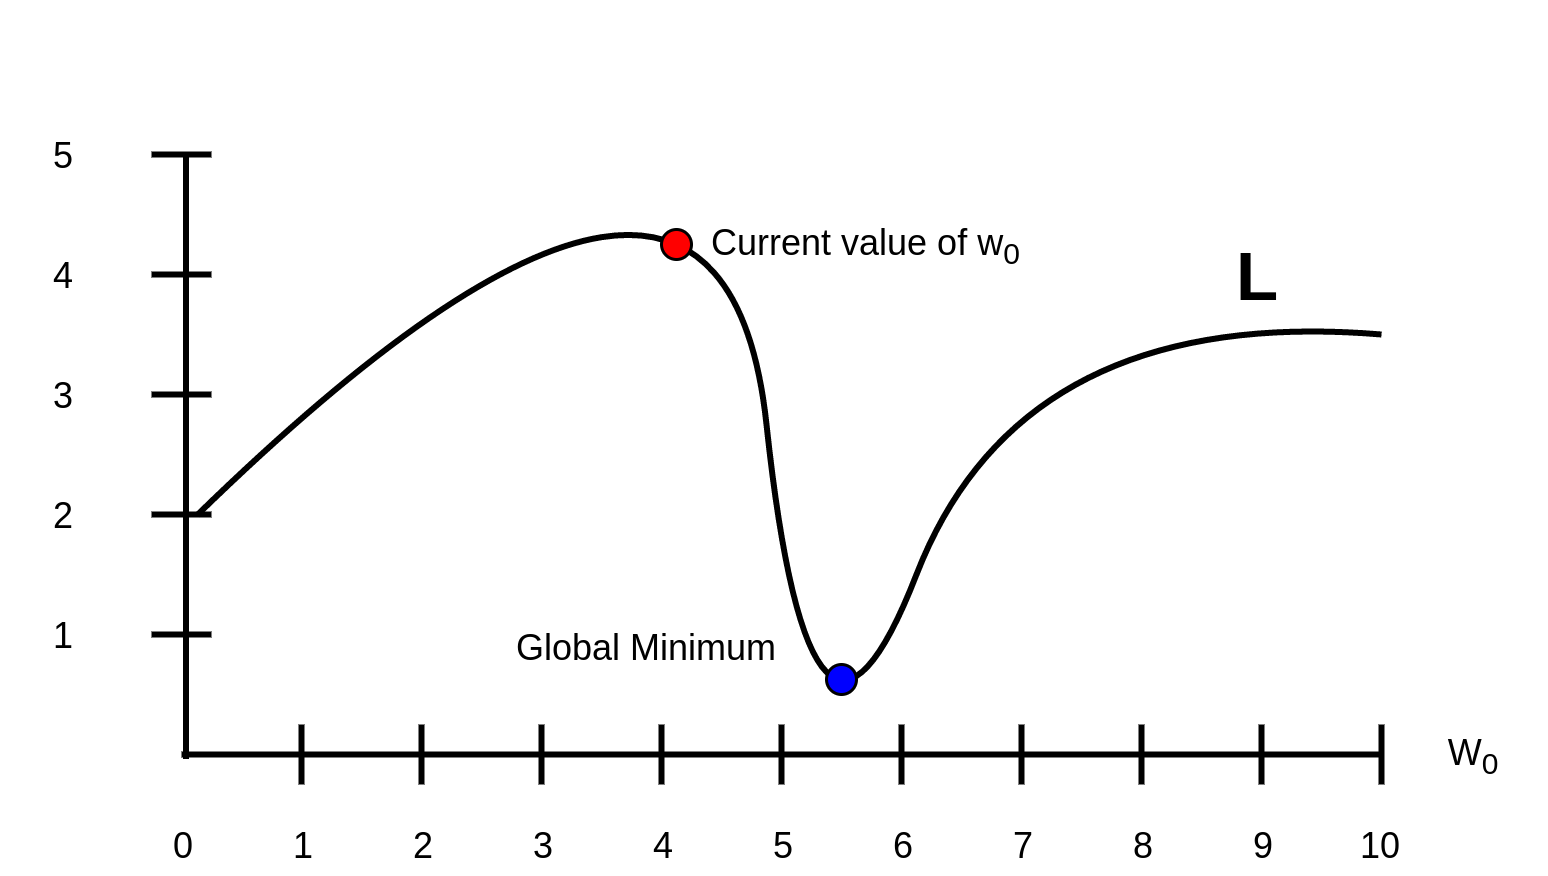
\includegraphics[width=\textwidth]{lossFunction0}
                        \end{figure}
                        
                        \par Now, as we adjust the weight (current red point), the magnitude of our loss function will alter. We can traverse that loss function by changing the weight w. If we change the weight w such that the value loss function decreases, this corresponds to having greater accuracy within our sample, since that is what the loss function captures.
                        
                        \par What gradient descent does is alter the weight in correspondence with the slope of the line. Take our current point, which is fortunately on the cusp of a precipice towards the global minimum of the loss function. The slope at this point is negative, meaning as the value of the variable on the x-axis increases, the value of the variable on the y-axis decreases. We are trying to descend towards the lowest point\footnote{Hence the term gradient descent.}, so a negative slope tells us we should increase the value of w to reduce the value of \textbf{L}.
                        
                        \par When we do so, we might get here (depending on some parameters):
                        
                        \begin{figure}[h]
                            \caption{Adjusted w.}
                            \centering
                            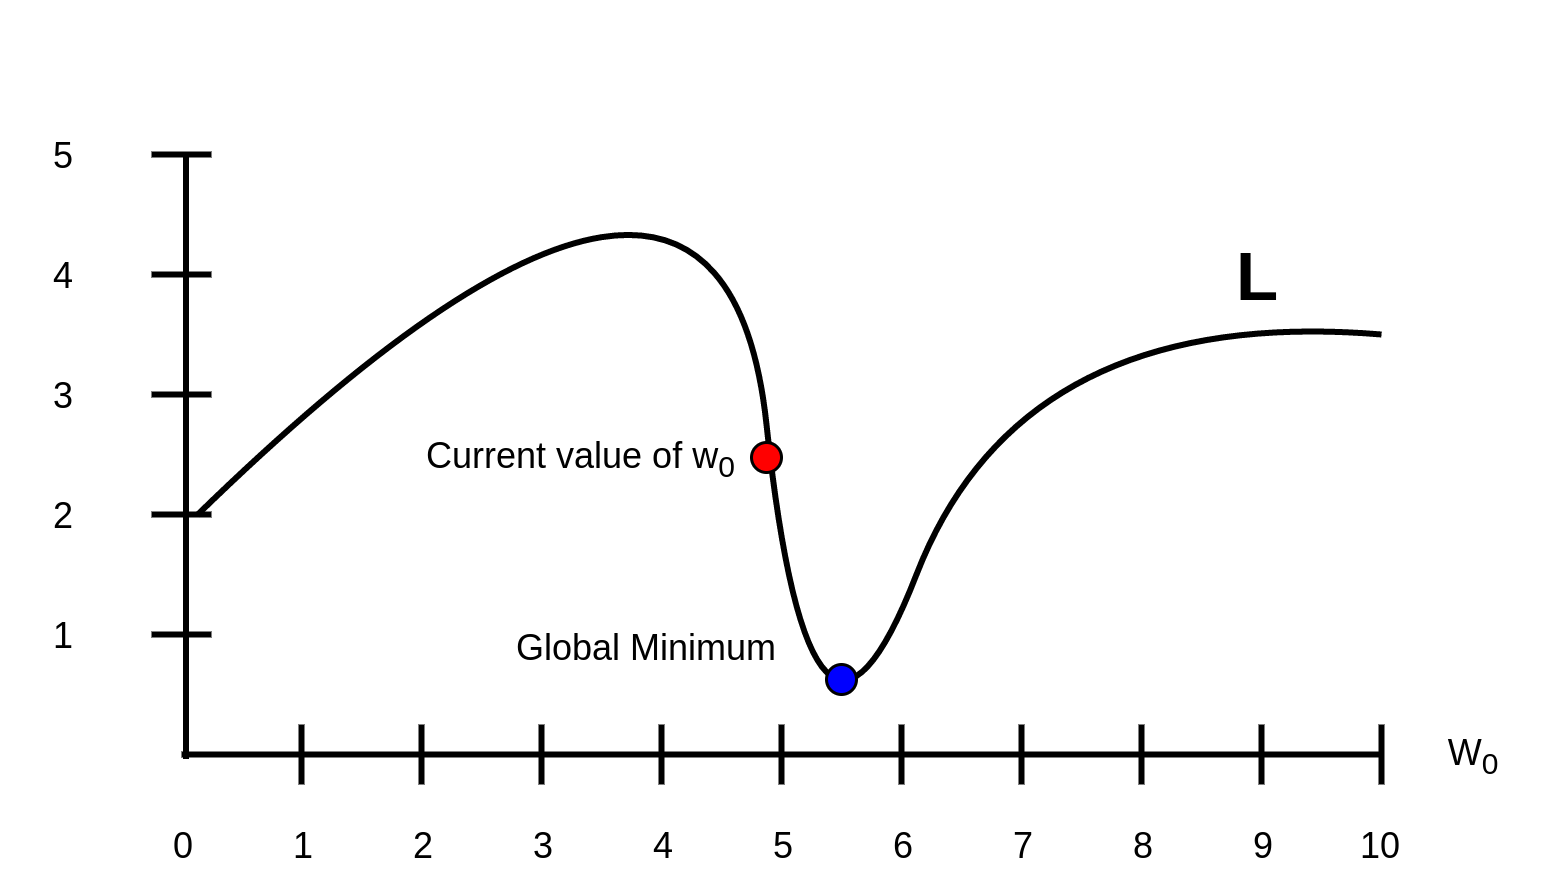
\includegraphics[width=\textwidth]{lossFunction1}
                        \end{figure}
                        
                        \par The iteration then continues until the slope is fount to be ~0 at the global minimum.
                        
                        \par This is a greedy algorithm, and one can see that should w\textsubscript{0} have been initialized to the value of 2 or so, the gradient descent algorithm would have taken it towards the left, rather than the right. Thus, gradient descent is susceptible to "local minima", or little kinks in the graph it may get stuck on. For more details, please see \cite{logisticRegression}\footnote{Relevant part starts at ~ 53:15 minute mark.}.
                        
                        \par Gradient descent is defined as follows:
                        
                        \par {\LARGE w\textsubscript{i} = w\textsubscript{i} - 
                        \(\alpha\)\(\frac{\partial L(W)}{\partial w\textsubscript{i}}\)}
                        
                        \bigskip
                        
                        \par To explain what is going on here. The w\textsubscript{i} is the weight we are currently adjusting, let us say the the weight that will be multiplier of the number of bedrooms in our neuron. The reason for the subscript i is because we may have a whole lot of these, one for each feature, and each of them will be updated differently, since the magnitude of the weights of each of the features will (hopefully) be different. So as we alter the weights, the weight for the number of bedrooms should hopefully increase in larger increments than the weight for the square footage.
                        
                        \par The \(\alpha\) there is the "learning step size". The larger the \(\alpha\), the greater the size of the updates to the weights will be. One may use a constant alpha, or one may reduce it as the number of updates thus far increases and so forth.
                        
                        \par Now that partial derivative, {\Large \(\frac{\partial L(W)}{\partial w\textsubscript{i}}\)}. As You can see, the derivative is of our function L, which should capture the performance of the neuron. The W is the set of all the weights (in our example neuron, this set is of size 5). The L is the function that we are trying to descend or ascend, as the case may be (descend if it is minus \(\alpha\), ascend if plus). Finally, the partial derivative is with respect to the current w\textsubscript{i}, since we want to see how does altering w\textsubscript{i} affect the value of the loss function.
                        
                        
                    \subsubsection{Training the Neuron}

                        \par All that is left is to apply gradient descent to the neuron and the weights. Unfortunately however, our threshold function is non-continuous and consequently non-differentiable. This is remedied by using a "soft" threshold\cite{mitNeuralNetwork}\footnote{Explained at 25:00 minute mark.}, which makes our neuron diagram look like:
                        
                         \begin{figure}[h]
                            \caption{A simple neuron, with a soft threshold.}
                            \centering
                            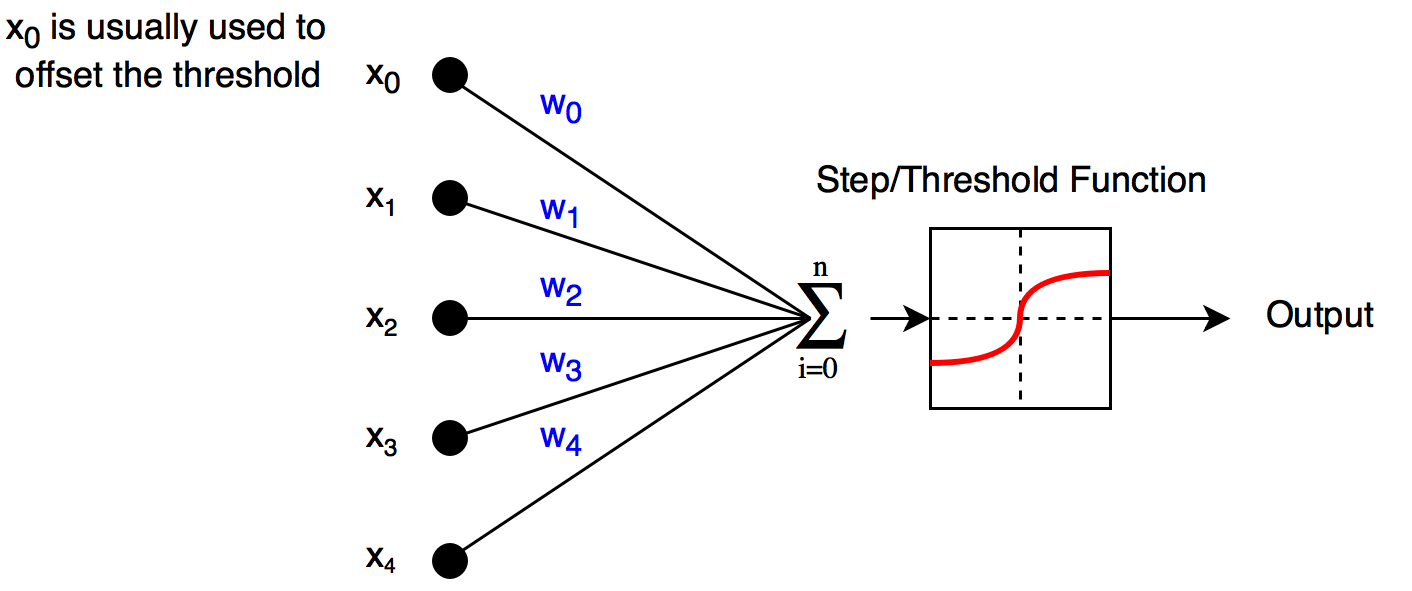
\includegraphics[width=\textwidth]{neuron2}
                        \end{figure}   
                        
                        \par The details of the differentiation can be found at \cite{logisticRegression}\footnote{Explained at the 25:00 minute mark, not a duplicate of above footnote.}, but the intuition should be sufficient for a general understanding.  
                        
                        \newpage
                        
                    \subsubsection{A Network of Neurons, or a Neural Network}                    
                    
                        \par Here is what a neural network looks like visually:
                        
                        \begin{figure}[h]
                            \caption{A neural network.}
                            \centering
                            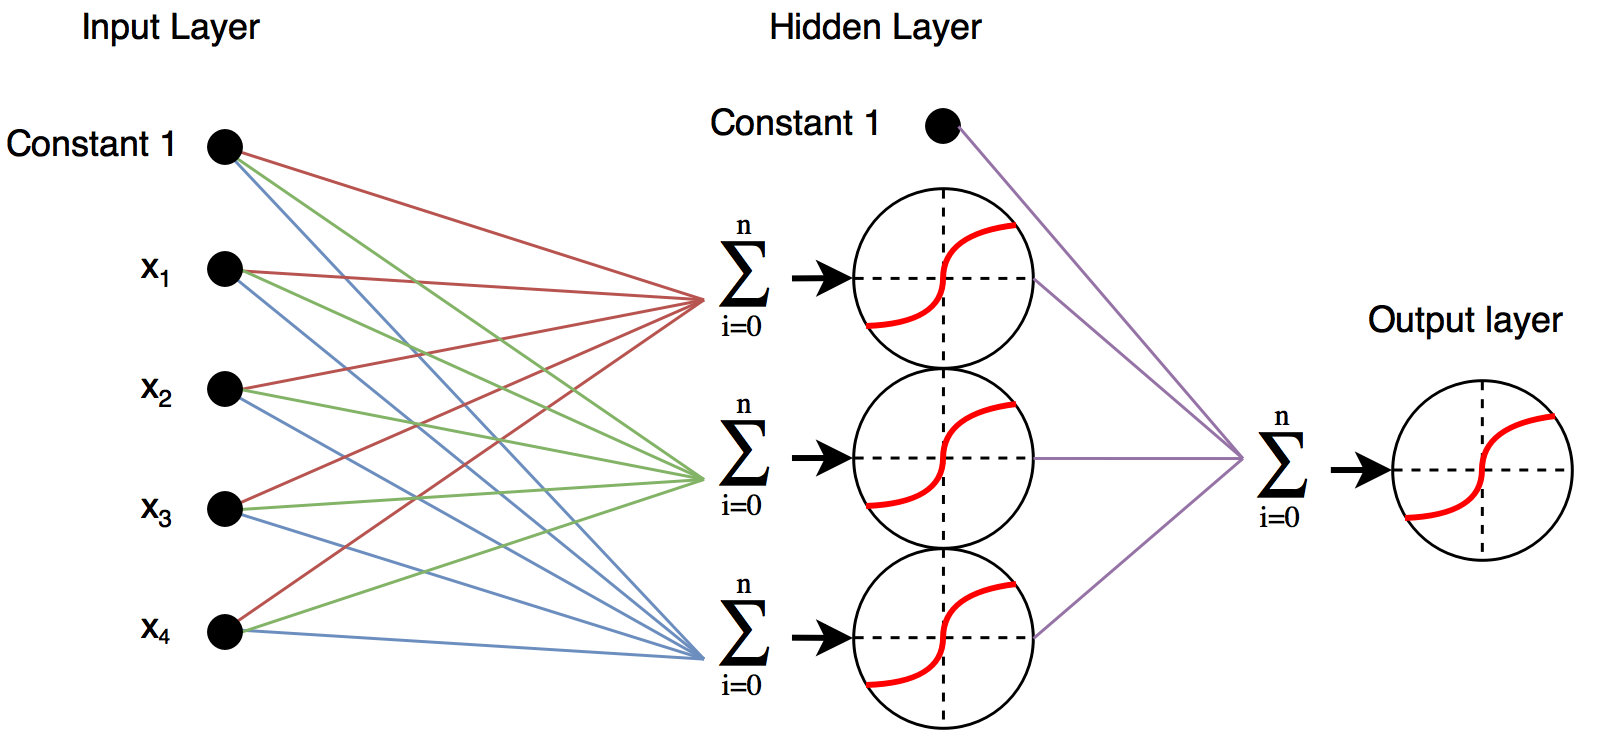
\includegraphics[width=\textwidth]{neuralNetwork}
                        \end{figure}  
                        
                        \par As the name would suggest, it is simply a network of neurons. 
                        
                        \par Note the "hidden" layer, so termed because it is not strictly visible to anyone outside the algorithm. Each of the outputs of the hidden layer have a weight attached to them, just as did the inputs. The network can consist of more than one hidden layer, and the number of neurons in each hidden layer may differ (giving rise to a technique known as autoencoding\cite{autoEncoding}).
                        
                        \par A neural network is trained with gradient descent (either stochastic or batch \cite{caltechNeuralNetwork}). However, a problem arises in the differentiation of the neural network, namely, how does one efficiently find the derivative of the entire neural net with respect to each of the weights w\textsubscript{i}? The change in some weight w\textsubscript{i} affects all downstream neurons, making the derivations very involved\footnote{Explained in much more detail in \cite{mitNeuralNetwork}, 43:00 minute mark.}.
                        
                        \par The answer is an algorithm named "backpropagation". A very broad overview is that by deriving from the output layer backwards (hence back propagation) we can re-use partial derivatives making the differentiation feasible. The algorithm is explained in great detail in \cite{caltechNeuralNetwork}, at the 33:00 minute mark.
                        
                        \par Otherwise, the process by which a neural network is trained is extremely similar to how a single neuron is trained: We are still just optimizing parameters, namely the weights, in order to minimize the value of the loss function, which minimization is done by using gradient descent. The core difference between training a neuron and a neural network is the specialized algorithm for generating derivatives with respect to each parameter, backpropagation.
                        
                      
                \newpage                  
                \subsection{Support Vector Machine}
                
                    \subsubsection{Intuition}
                    
                        \par There are two core ideas behind support vector machines: optimal linear separators and kernel functions.
                        
                    \subsubsection{Optimal Linear Separator}
                    
                        \par Picture the following two-dimensional training set:
                        
                        \begin{figure}[h]
                            \caption{A linearly separable set.}
                            \centering
                            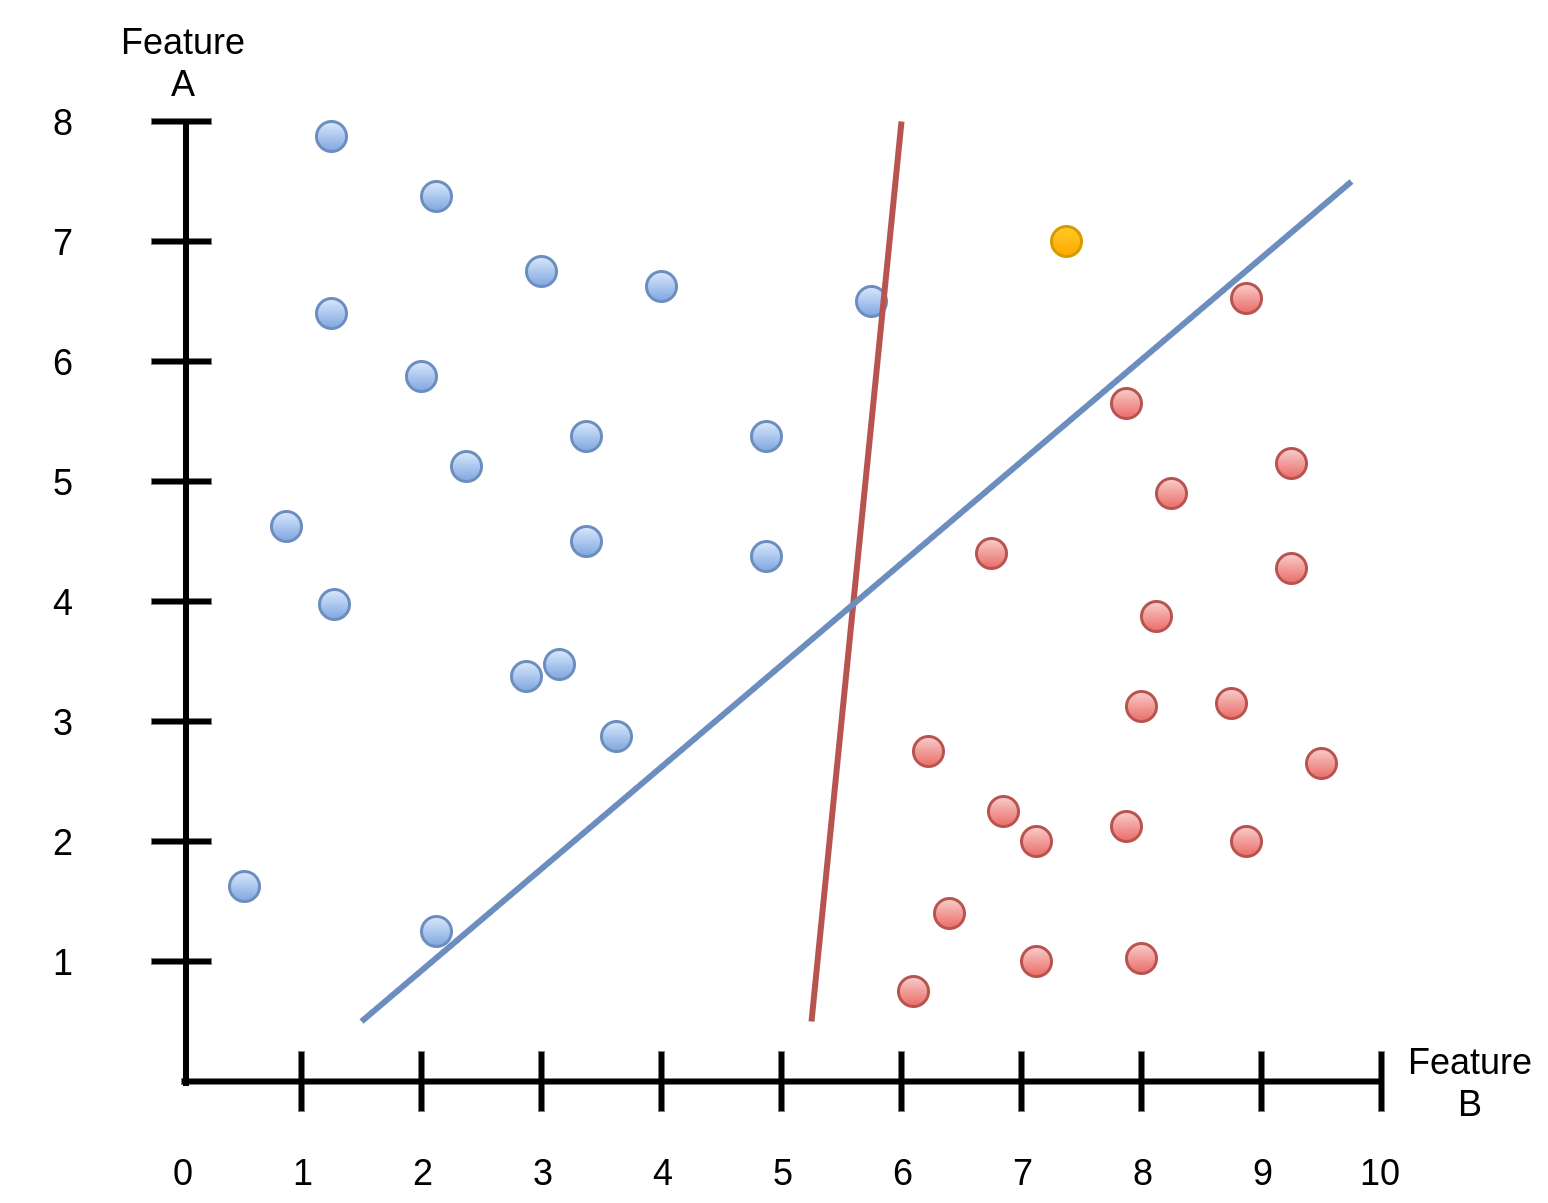
\includegraphics[width=\textwidth]{poorClassifiers}
                        \end{figure}  
                        
                        \par The above is a "linearly separable" set, which simply means that the blue points and the red points can be separated by a straight line\footnote{Which, straight lines are linear functions, hence the term linearly separable.}. 
                        
                        \par In the figure, there are two linear separators, the blue and the red. Each gives a different classification to the newly observed sample, which is in gold. Which is the better linear separator? Furthermore, an infinite number of possible separators exist, rather than just the two pictured. How would one go about picking the "best one", and what metric would one use to decide?
                        
                        \par One idea is to try to make a separator that puts as much space between the two clusters (red and blue) as possible, in hopes that that will most faithfully capture the underlying relationship. That separator looks something like:
                        
                        \begin{figure}[h]
                            \caption{A better classifier, allegedly.}
                            \centering
                            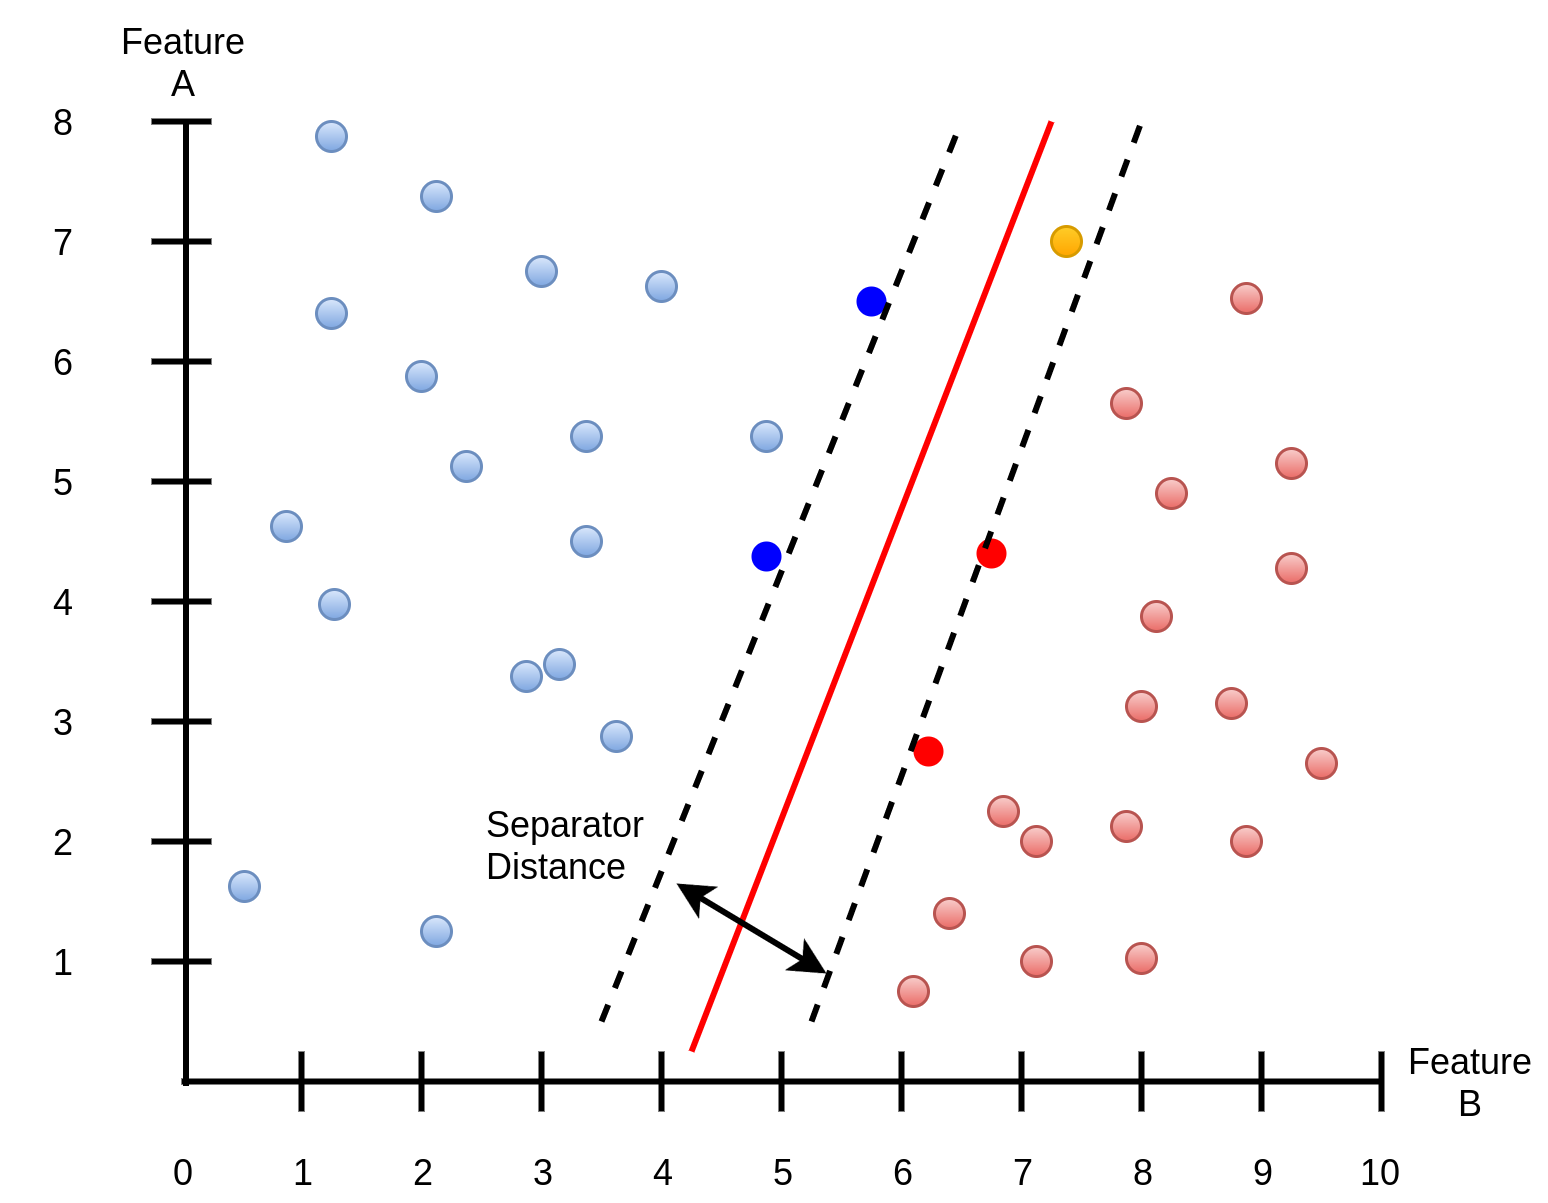
\includegraphics[width=\textwidth]{betterClassifier}
                        \end{figure} 
                        
                        \par To explain some of what is going on there. Picture that the punctuated lines are the edges of a road, and that the red separator in between them marks the center of the road.\footnote{This pedagogical device is from \cite{mitSupportVectorMachine}} The wider we can make this road, the greater the separation between the two clusters, the more our effective our linear separator should be on newly observed data.
                        
                        \par There are two points in saturated blue, and two points in saturated red. Those are the "support vectors"\footnote{Hence the name, Support Vector Machine.}. They define how our linear separator in red was drawn, since they are the ones forming the boundaries of our street. 
                        
                        \par That's one of the two core ideas: draw the "best" line You can to separate the sample. But what if the sample is not linearly separable, namely, no straight line can separate the red and blue points? That's where kernel functions step in.\footnote{Not quite. More on that in the next section.}
                        
                        \par A from the ground derivation for support vector machines can be found at \cite{mitSupportVectorMachine} and \cite{caltechSupportVectorMachine}.
                        
                    \newpage
                        
                    \subsubsection{Soft-Margin SVMs}
                    
                        \par In the previous graphs, we had a neatly linearly separable training set. Such sets, however, are seldom seen in the real world. Broadly speaking, there are two main cases of non-separability: mild and severe.
                        
                        \par Below is an example of \textit{very} mild inseparability:
                        
                        \begin{figure}[h]
                            \caption{A \textit{very} mildly inseparable set.}
                            \centering
                            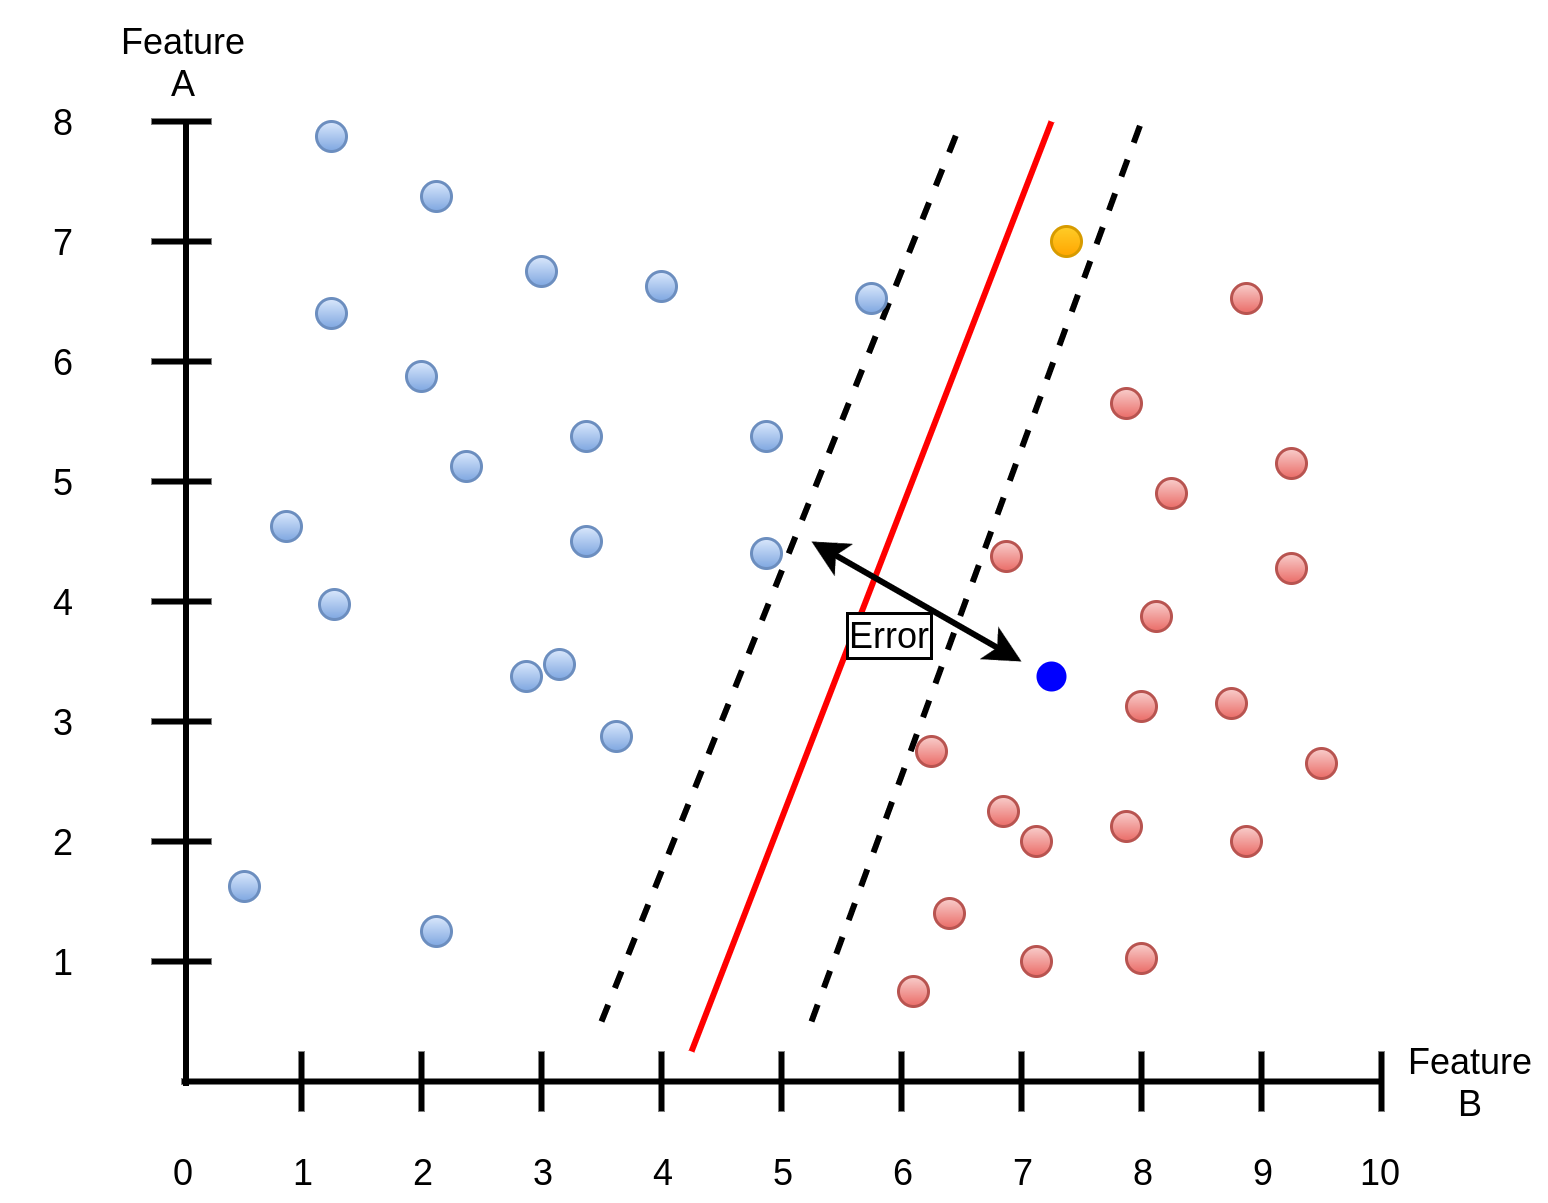
\includegraphics[width=\textwidth]{mildlyInseparable}
                        \end{figure} 
                        
                        \par The offending point is in bold blue. Now, it is quite apparent that the bold blue sample is over-all just an outlier, and that even though it might be reasonable to shift our separator a little, completely altering it would be ill-advised.
                        
                        \par The solution is as follows: in the original, linearly separable case, we were trying to optimize for the widest possible division of the sample clusters in question. We should keep that, since that is the core of SVMs, but let's add in an "error" for every point. If the point is on the correct side of the linear separator, as well as outside the "road"\footnote{The road is delineated by the dotted lines, and represents the width of the separation of the clusters.}, then it's error is 0. Otherwise, the error is the distance between the correct side of the "road" and the sample point. Take for example the point in bold blue. The error is from the left dotted line to the point, since the bold blue point \textit{should} be able to the left of the "road".
                        
                        \par To get the total error, simply sum the error of all points in the training set relative to the "road".
                        
                        \par Now, instead of only optimizing for the width of the separation between our clusters, we simultaneously optimize for a trade-off between the greatest width and least error. This, however, introduces another parameter, namely, how important do we consider errors to be. This is a parameter to be optimized on a problem-per-problem basis. This notion is explained in detail in \cite{kernelMethods}.\footnote{46:00 minute mark.}.
                        
                    \newpage
                        
                    \subsubsection{Non-Linear Transformations and Kernel Functions}
                    
                        \par We've dealt with linearly separable and mildly linearly inseparable training sets. What about severely inseparable training sets?
                        
                        \begin{figure}[h]
                            \caption{A severely non-linearly separable training set.}
                            \centering
                            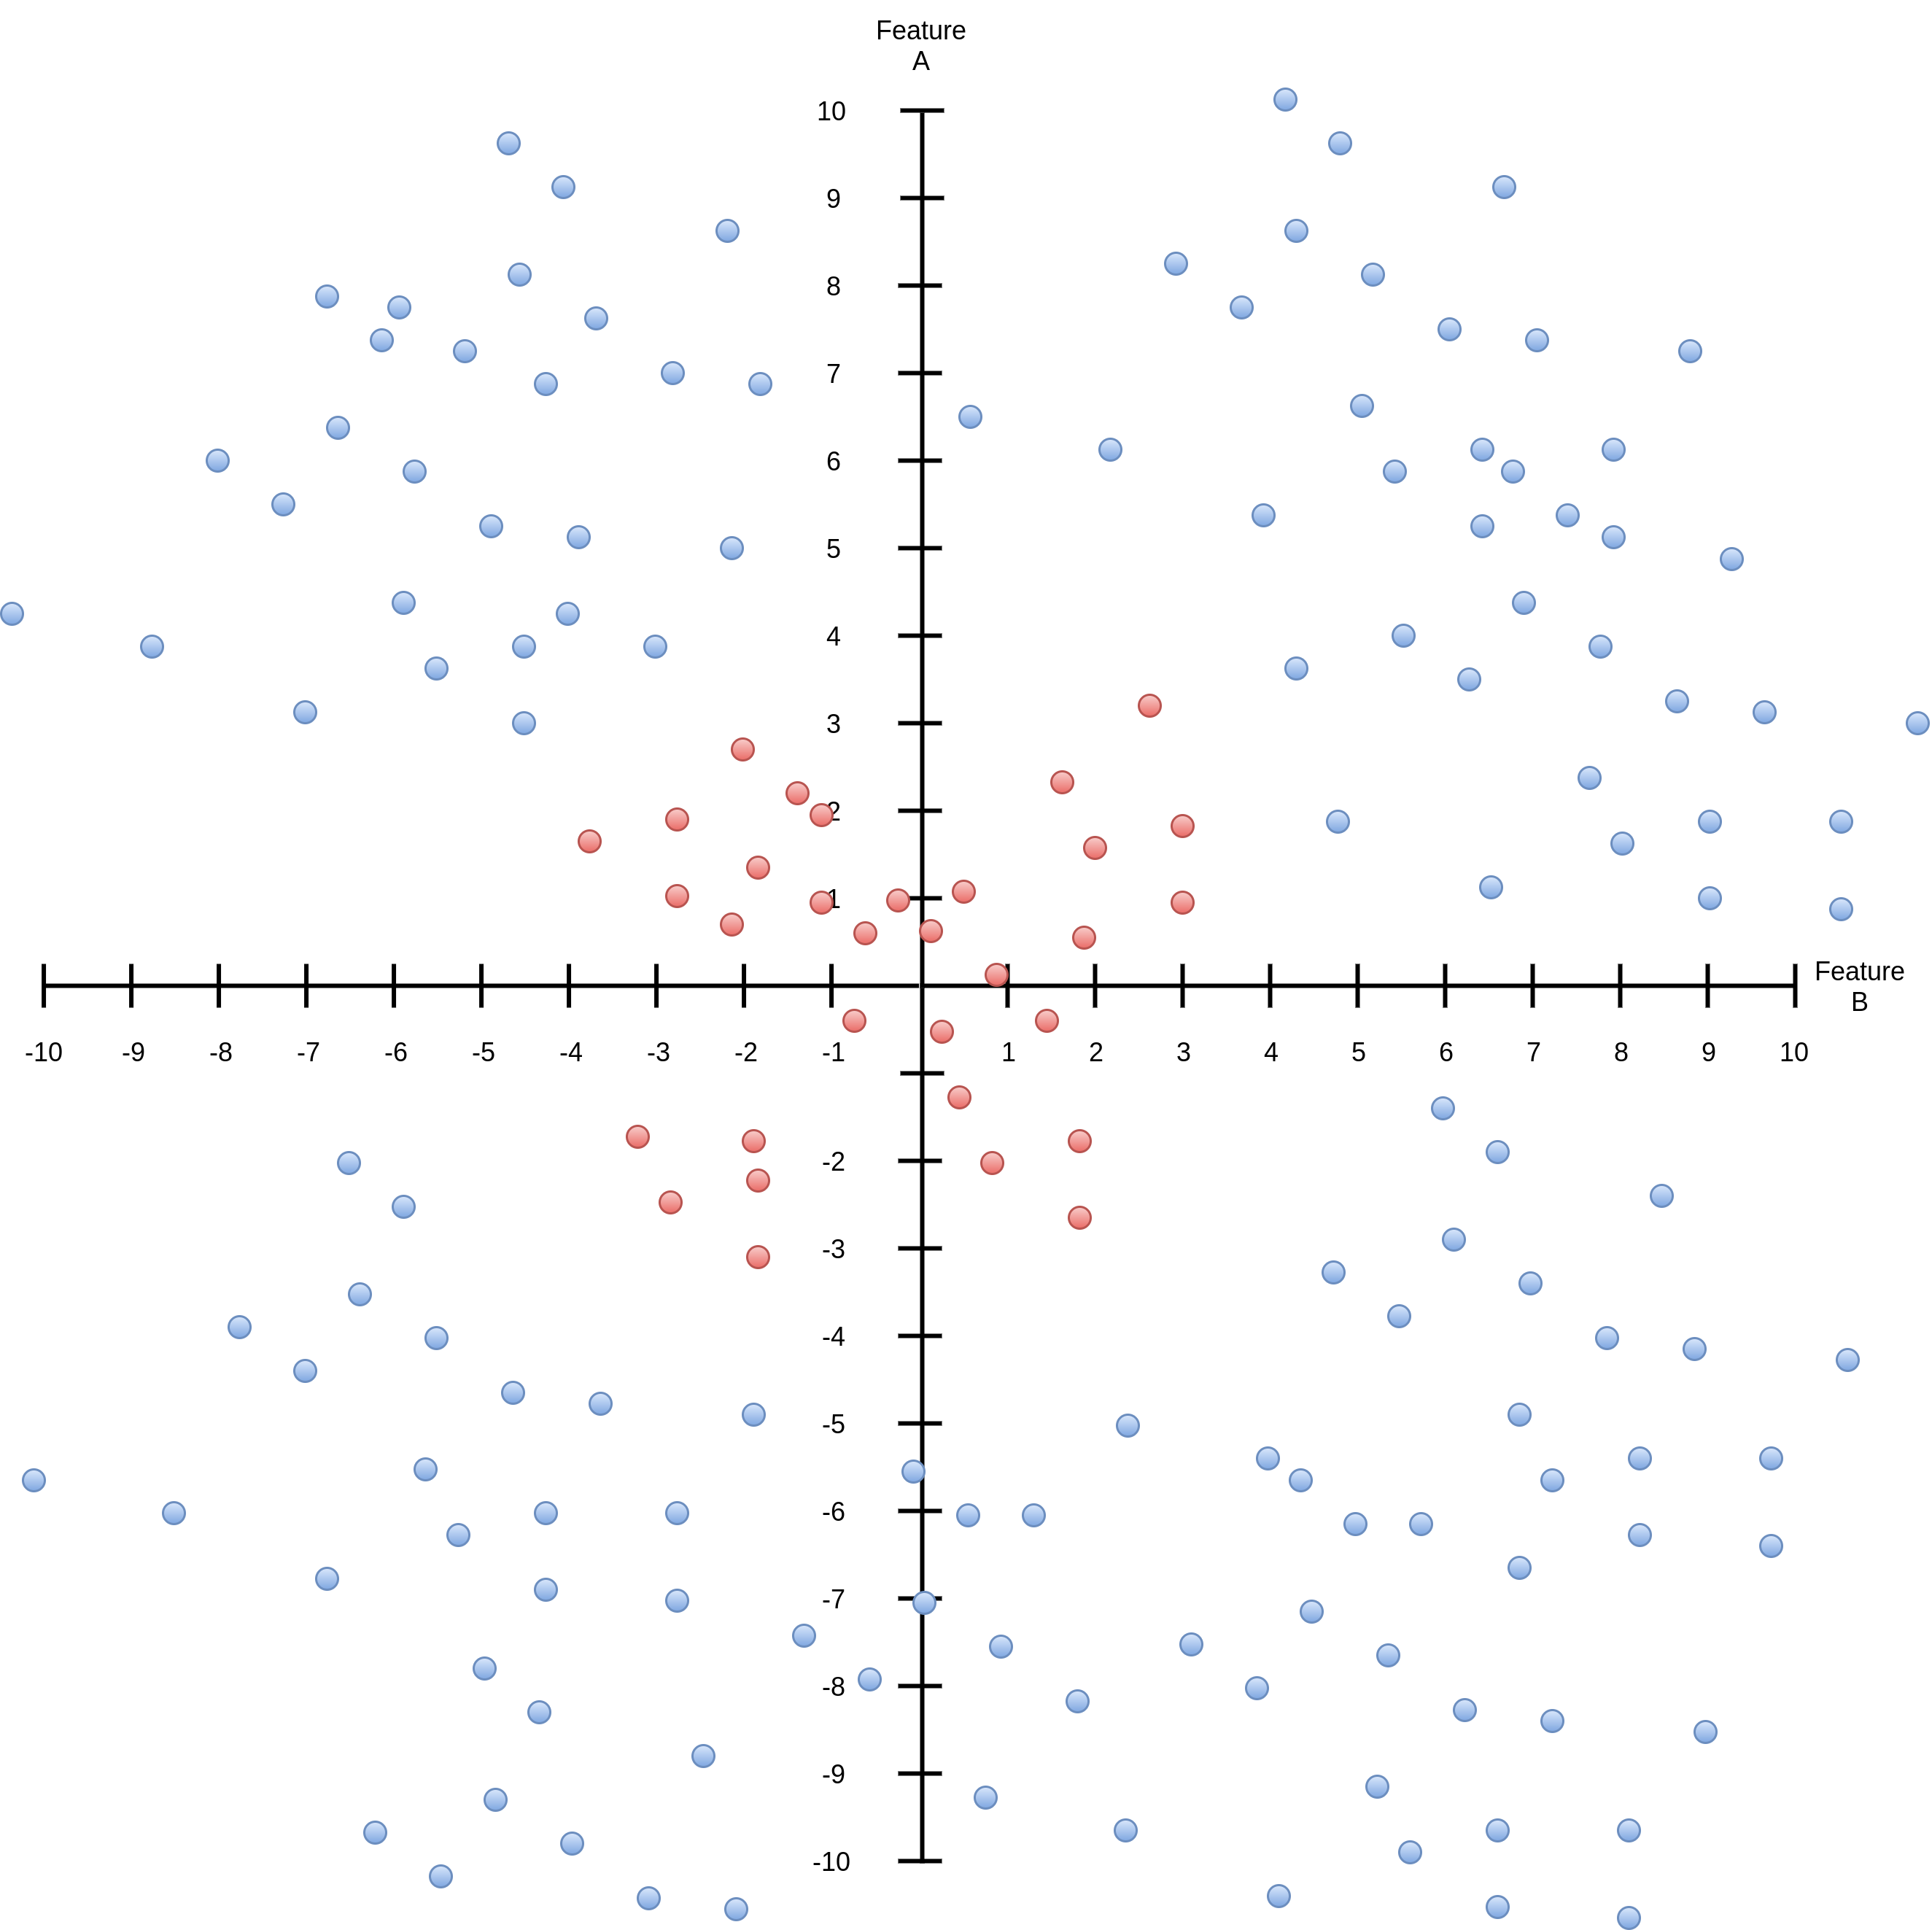
\includegraphics[width=\textwidth]{preTransformationSpace}
                        \end{figure} 
                        
                        \par No straight line can separate the above set in a satisfactory fashion, and all is lost for a support vector machine which tries to work in the above space. 
                        
                        \par A solution is to take the above the above set and apply a transformation to each point. In this two dimensional case, each point has an \textit{x} and a \textit{y} co-ordinate. A possible transformation then is, for each point, to square both of the co-ordinates, namely (\textit{x}, \textit{y}) \(\mapsto\) (\textit{x\textsuperscript{2}}, \textit{y\textsuperscript{2}}). This would transform the above set to:
                        
                        \begin{figure}[h]
                            \caption{Non-linearly transformed space.}
                            \centering
                            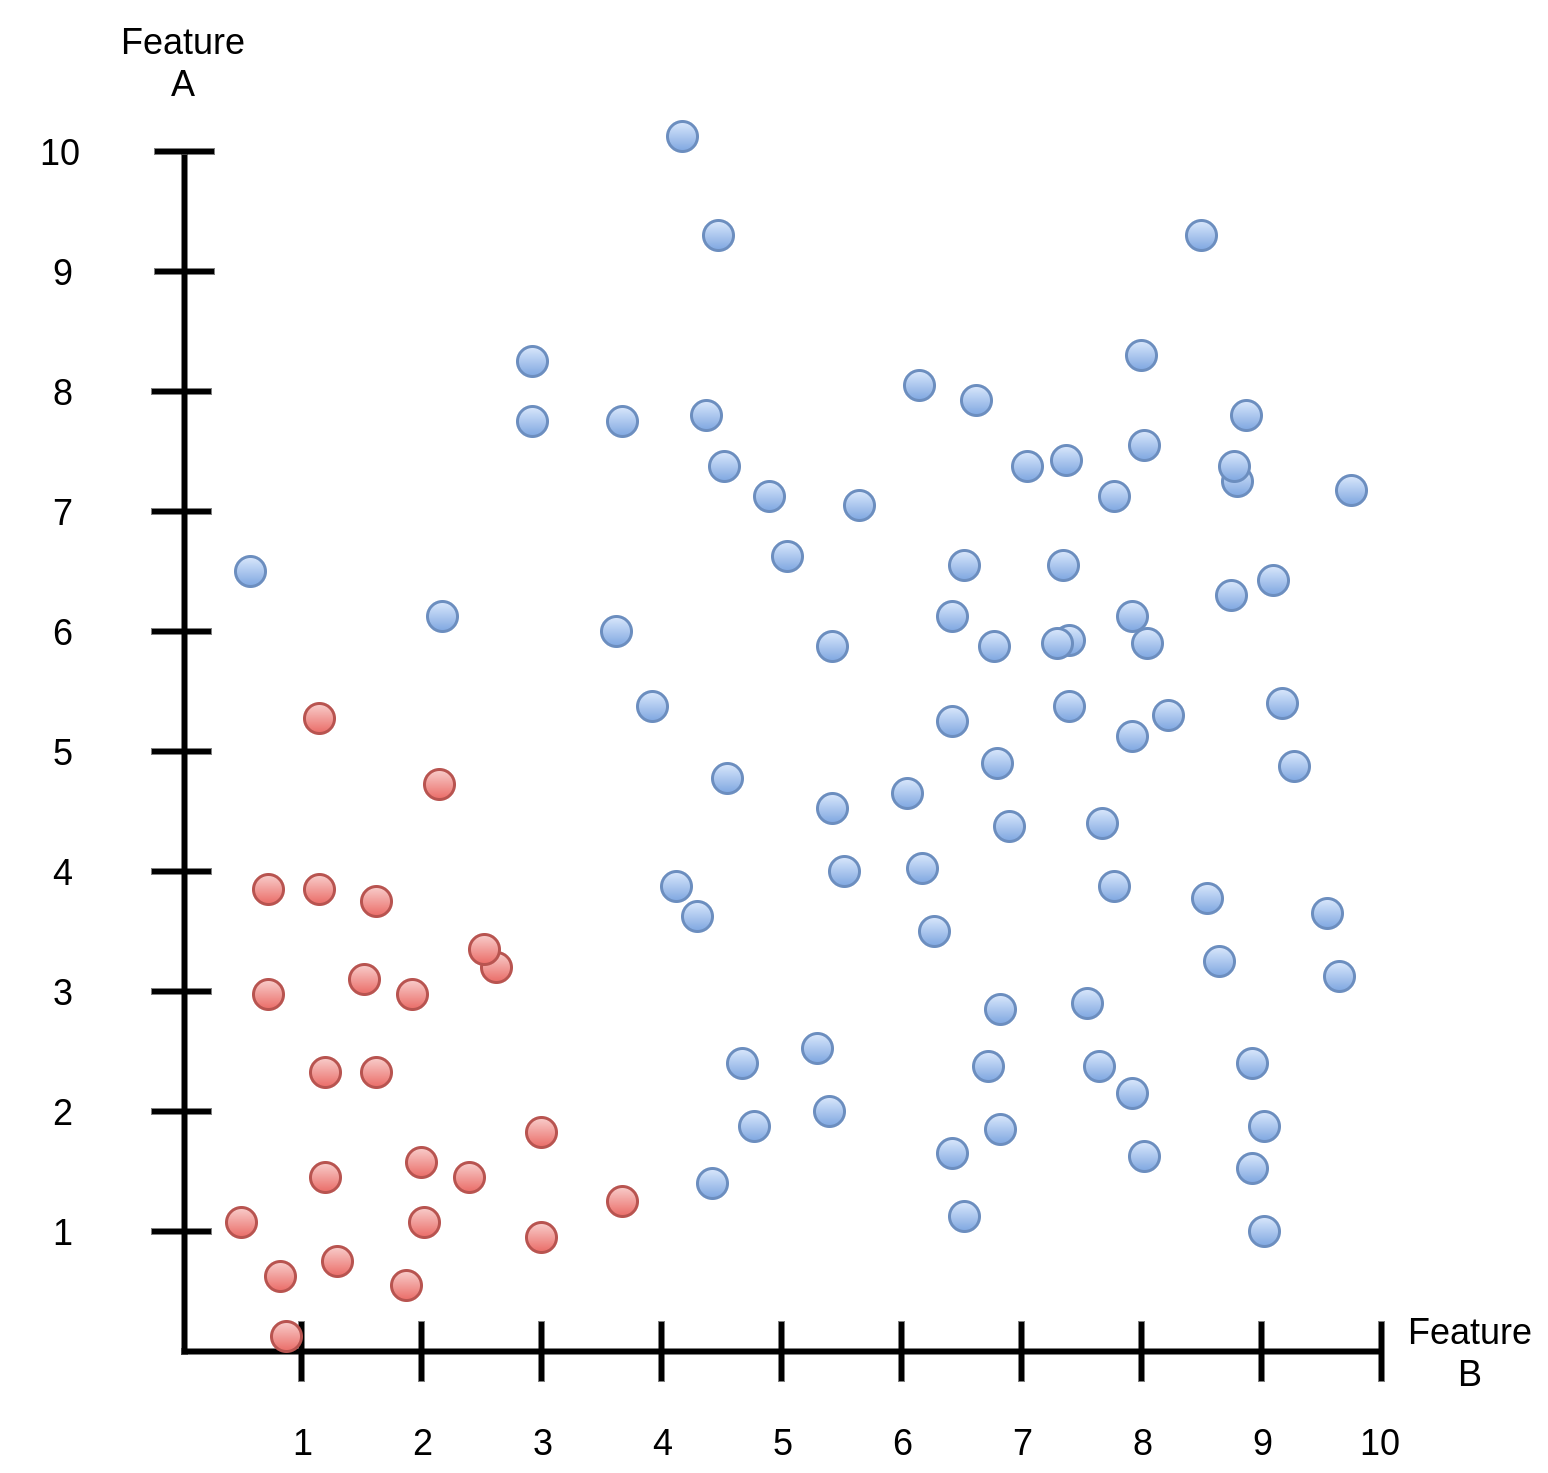
\includegraphics[width=\textwidth]{postTransformationSpace}
                        \end{figure} 
                        
                        \par The points from top left, bottom left, and bottom right quadrants have been translated to the top right quadrant as a consequence of the transformation\footnote{Squaring values ensures that the result is positive, hence the top right quadrant}, whilst their distance from the origin was preserved, resulting in a mildly inseparable case which soft margin SVMs would be able to handle.
                        
                        \par Kernel functions are these non-linear transformations, mathematically adjusted to exploit some naturally occurring mathematical conveniences to make them more powerful in SVM context.\footnote{Namely, SVM optimization is dependent solely on the dot product between SVM parameters and the training samples, which allows for some trickery.}. The particulars can be found at \cite{kernelMethods}\footnote{Beginning at the 06:00 minute mark.}.
                        
                        
                \newpage                  
                \subsection{Boosting}
                
                    \par There core idea behind boosting is the combination of a number of \textit{weak classifiers} to form a \textit{strong classifier}.
                    
                    \par A weak classifier is a classifier which, according to some performance measure, classifies samples correctly about 50\% of the time. Similarly, a strong classifier is a classifier which correctly classifies samples almost 100\% of the time.
                    \begin{figure}[h]
                            \caption{Weak and strong classifiers.}
                            \centering
                            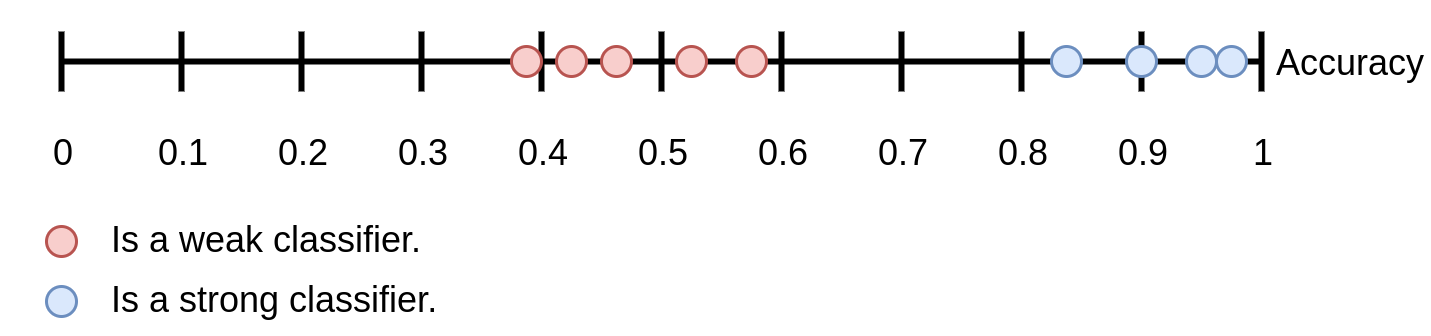
\includegraphics[width=\textwidth]{weakStrongClassifiers}
                    \end{figure} 
                    
                    \newpage
                    
                    \par A question arises: Can a series of weak classifiers be combined to form a strong classifier? Let the notion be illustrated via an example. Picture the following training set:
                    
                    \begin{figure}[h]
                            \caption{Training set.}
                            \centering
                            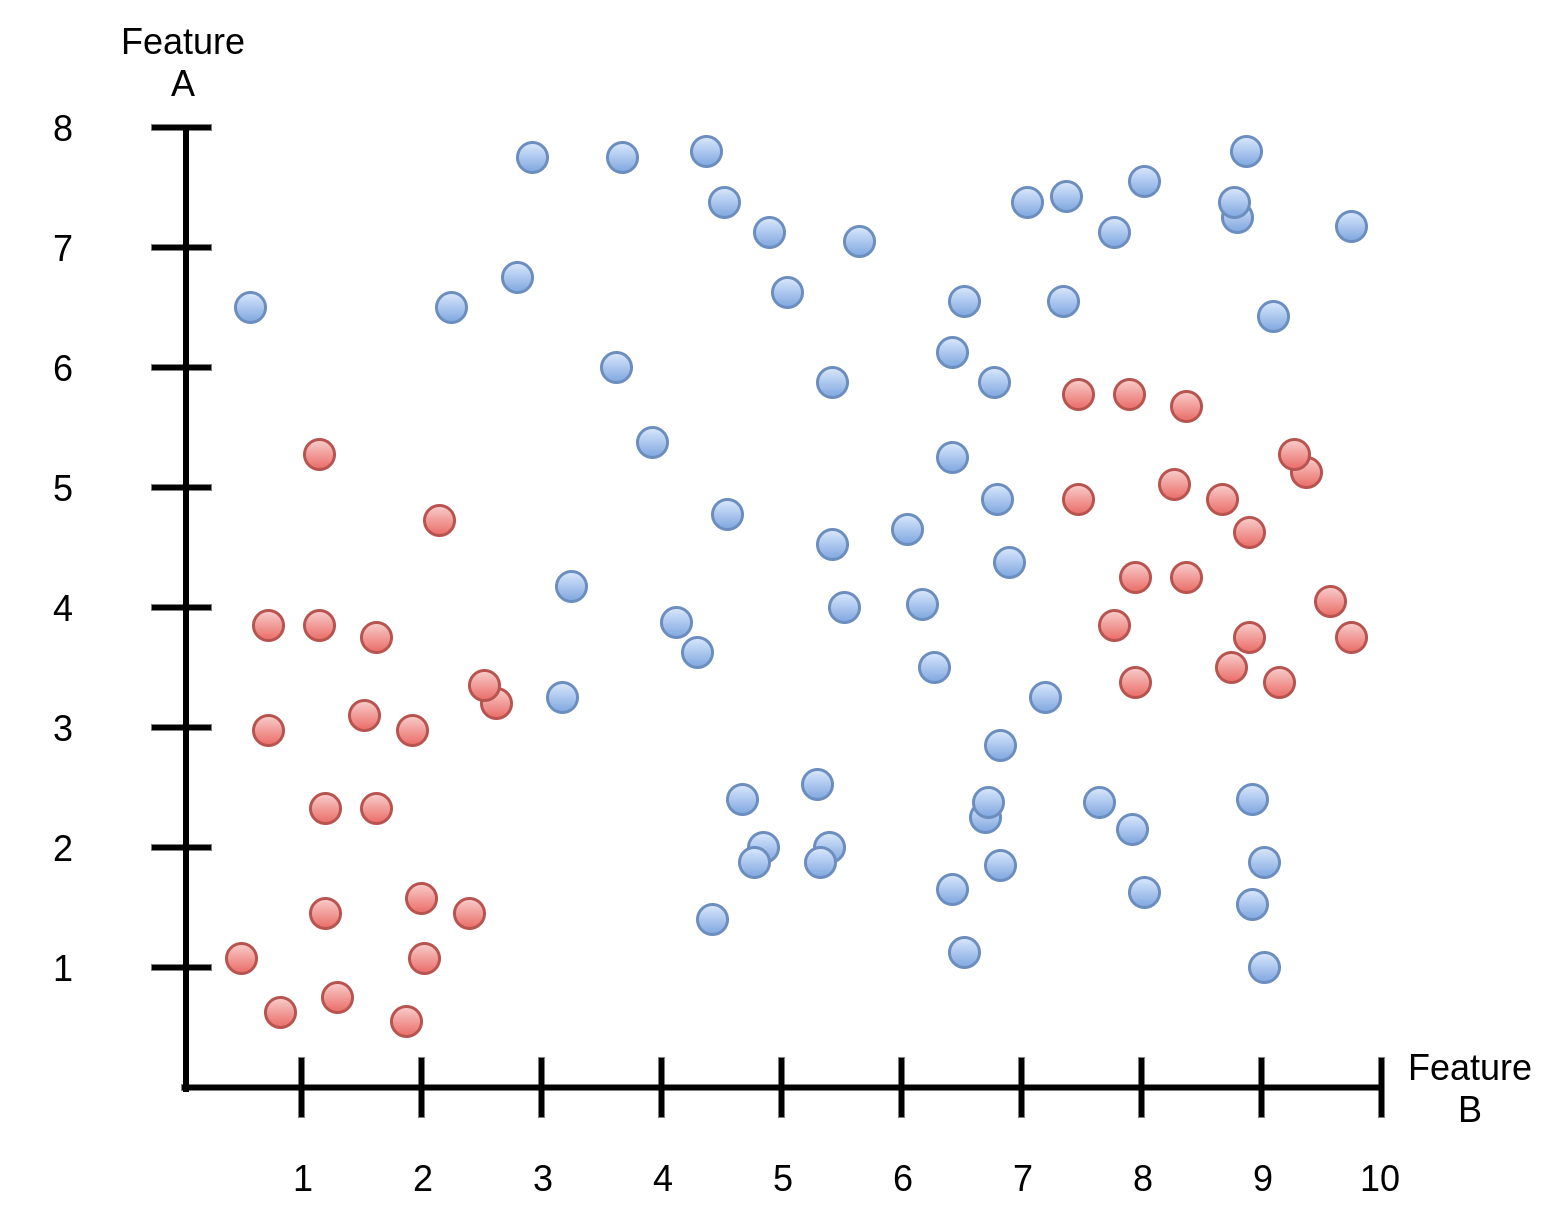
\includegraphics[width=\textwidth]{boosting0}
                    \end{figure} 
                    
                    \par Let us associate a weight w\textsubscript{i} with each of the samples, with all of the weights being equal at the beginning. From now and throughout every step, the weights will be assigned such that the summation of all of the weights sums to 1, namely: {\Large \(\sum\limits_{i}w\textsubscript{i} = 1\) }\footnote{This is to keep the weights as representative of a distribution, more details at \cite{boosting}, ~20:00 minute mark.}
                    

                    
                    \par In the search for a weak classifier, let us limit ourselves to horizontal and vertical linear separators.\footnote{Namely, decision tree stumps. If You'd like to know all there is to know about decision trees, see \cite{decisionTrees}}
                   
                    
                    \begin{figure}[h]
                            \caption{The first weak classifier.}
                            \centering
                            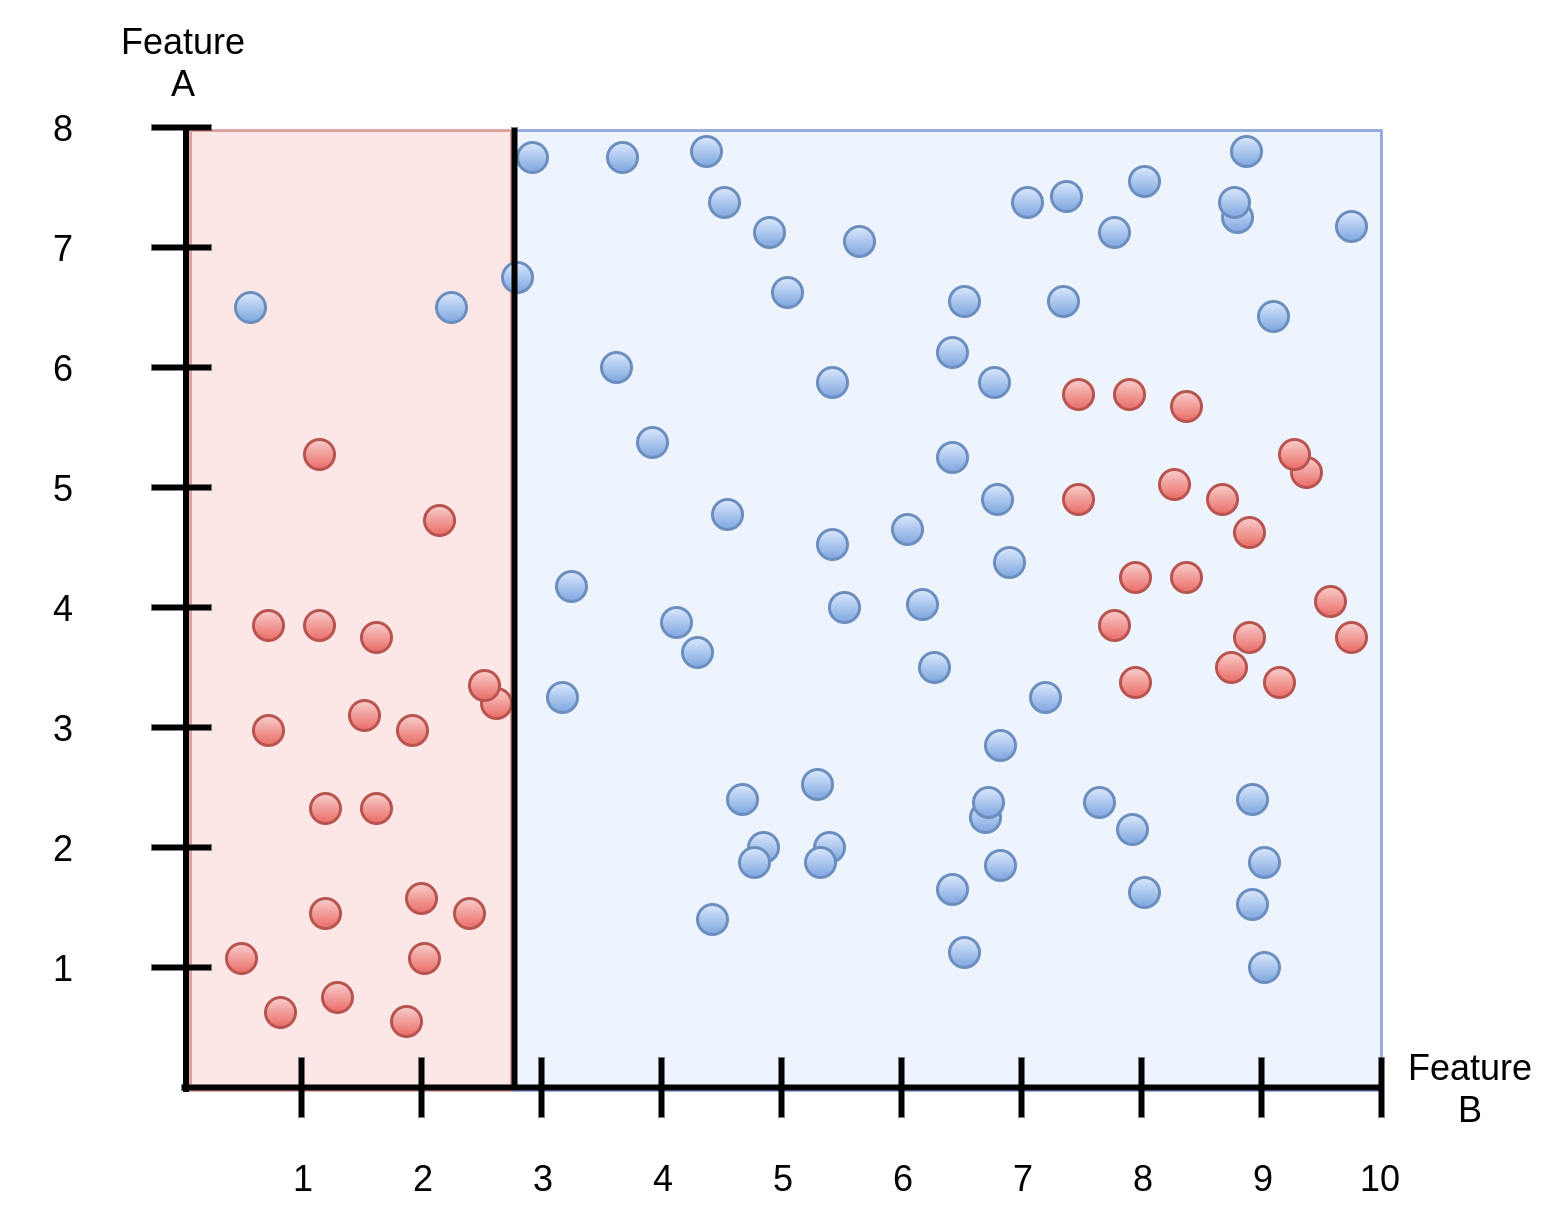
\includegraphics[width=\textwidth]{boosting1}
                    \end{figure} 
                    
                    \par Above, we created a horizontal linear separator at ~2.8 mark. The classifier claims that everything to it's left is a red point, and that everything to the right is blue. We are going to assign another weight, not to be confused with the weights we've already assigned to each of the samples (which are all currently equal), to our newly created classifier. The greater the accuracy of our weak classifier, the greater it's weight, since it makes sense to pay more attention to what this classifier has to say.
                    
                    \par Whilst most of the points are correctly classified, some of those blue points to the left, and all of those red points to the right are mis-classified. Now we are going to alter the weights of the samples, and increase the weights of the samples which were misclassified. To reflect this, their colouring is increased in intensity\footnote{Since the sum of all weights is to be kept a constant 1, an increase in weight of incorrectly classified points is equivalent to a decrease in the weight of the correctly classified ones.}:
                    
                    \begin{figure}[h]
                            \caption{Altered sample weights.}
                            \centering
                            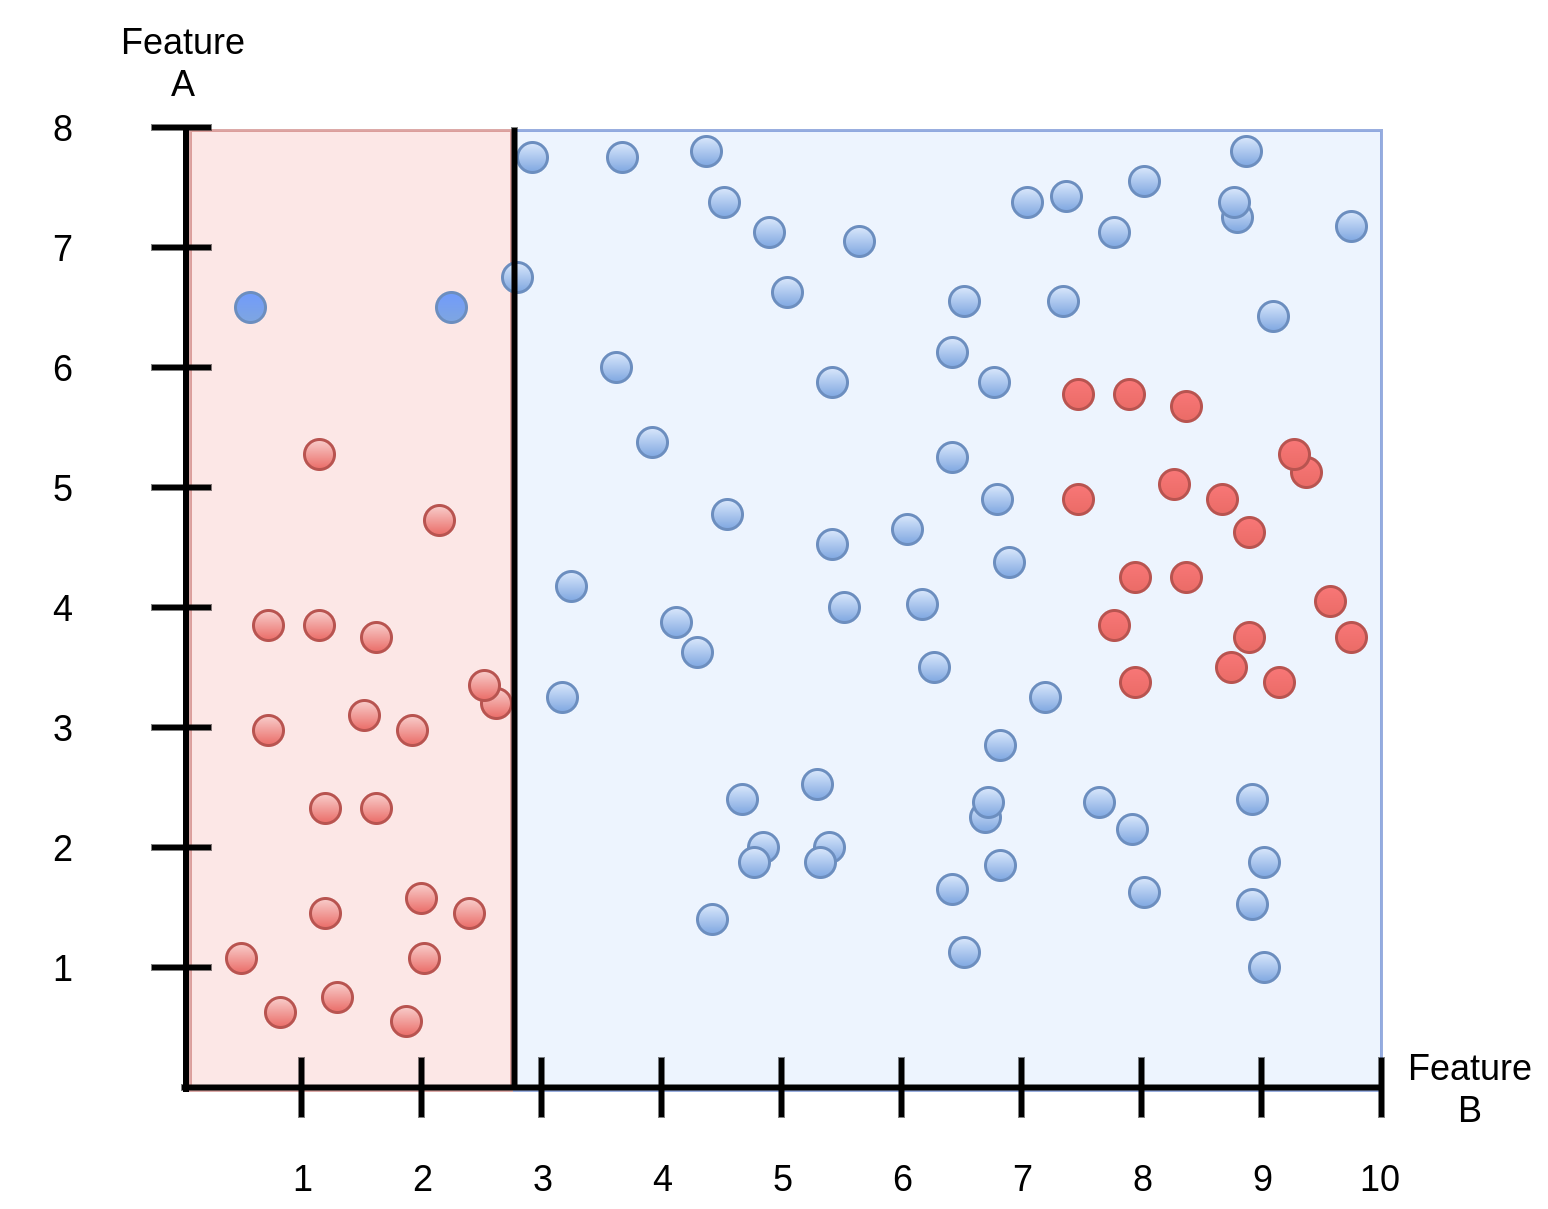
\includegraphics[width=\textwidth]{boosting2}
                    \end{figure} 
                    
                    \newpage
                    
                    \par Now we introduce another weak classifier, for instance:
                    
                    \begin{figure}[h]
                            \caption{The second weak classifier.}
                            \centering
                            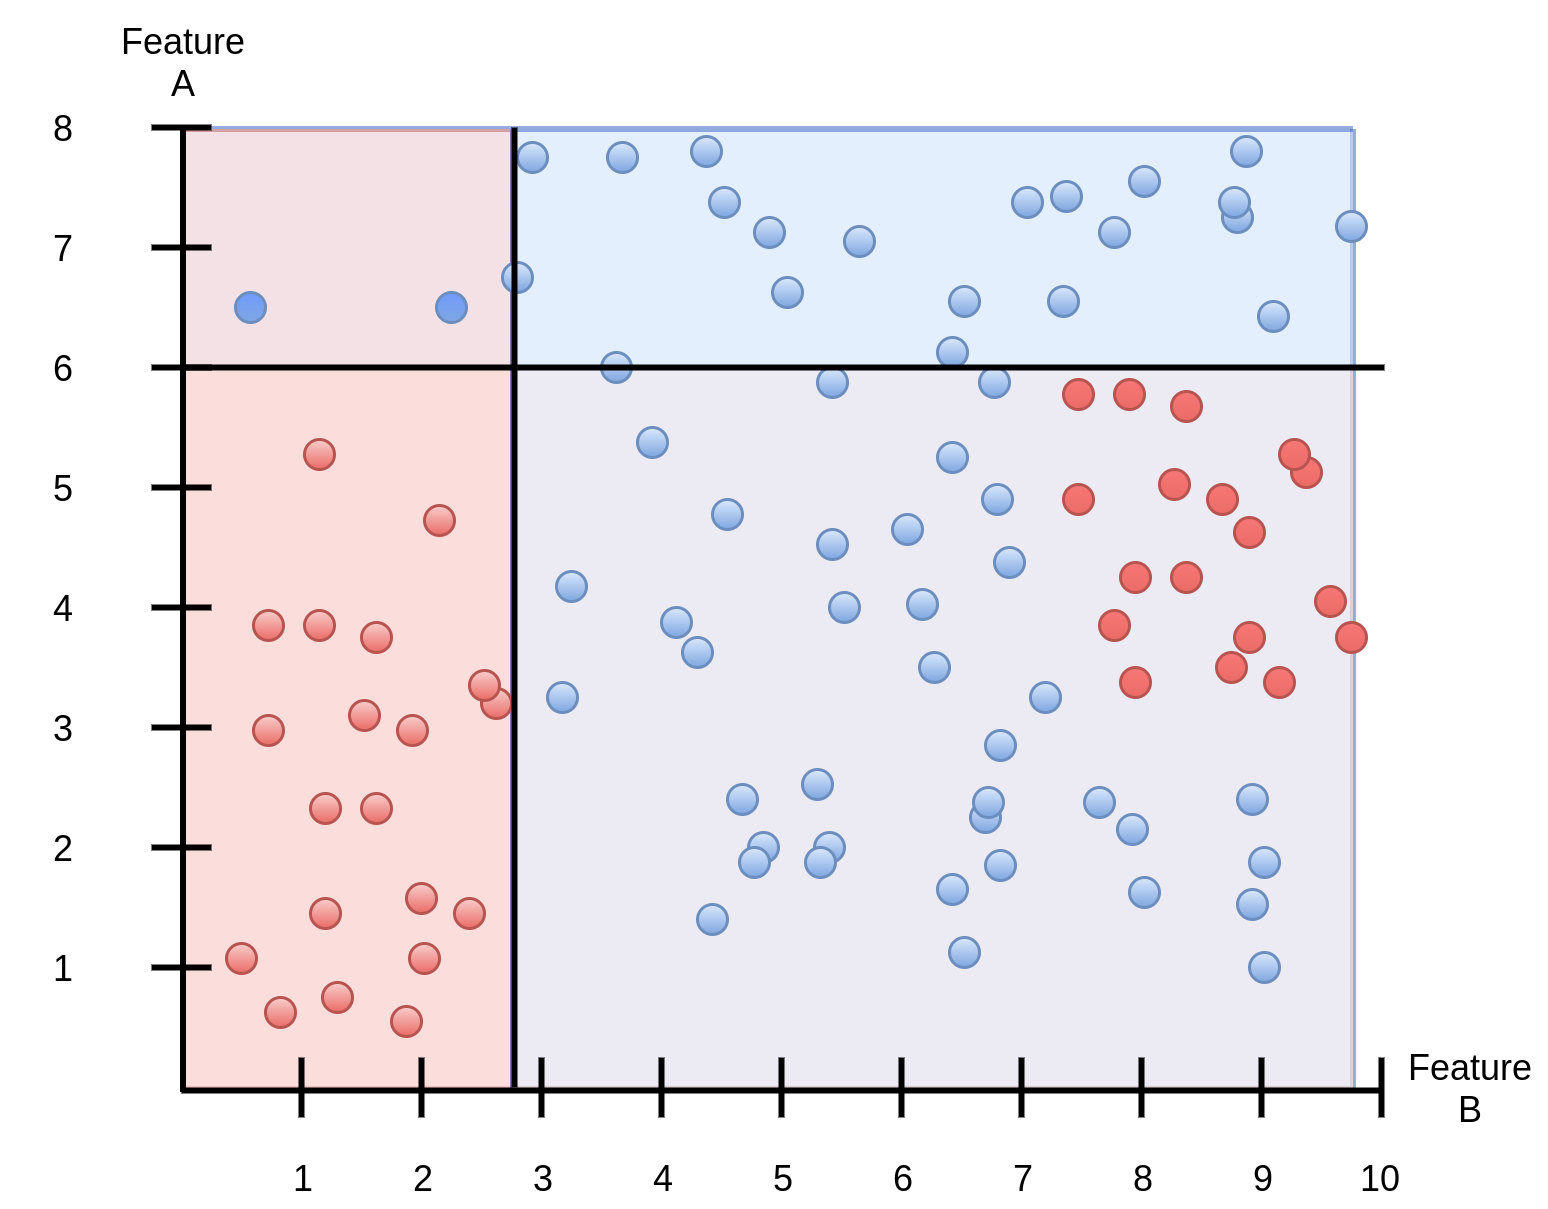
\includegraphics[width=\textwidth]{boosting3}
                    \end{figure} 
                    
                    \newpage
                    
                    \par The new weak classifier suggests that everything over 6 on the y-axis should be classified blue, and everything less than 6 should be red. Again, we assign a weight to the second classifier in accordance to how well it has performed. The importance is now shifted the freshly misclassified blue points as follows:
                    
                    \begin{figure}[h]
                            \caption{Again altered weights.}
                            \centering
                            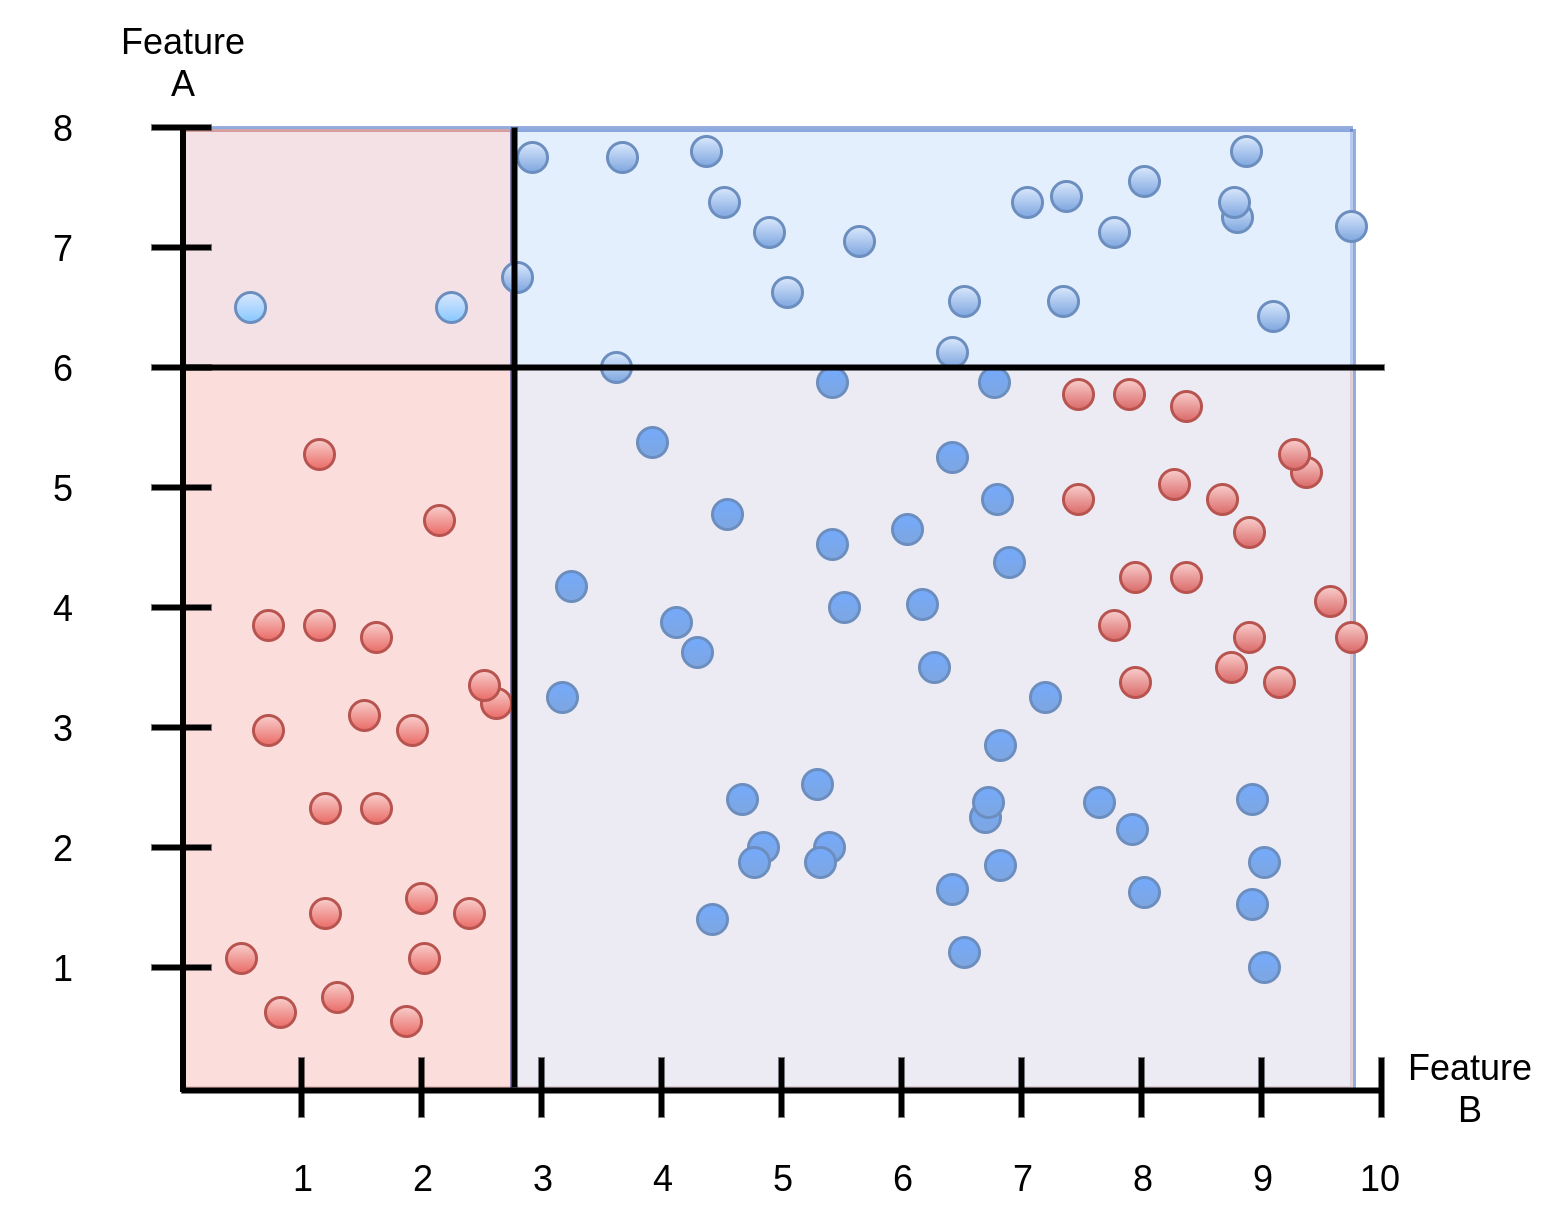
\includegraphics[width=\textwidth]{boosting4}
                    \end{figure} 
                    
                    \newpage
                    
                    \par Now for the third weak classifier:
                    
                    \begin{figure}[h]
                            \caption{The third weak classifier.}
                            \centering
                            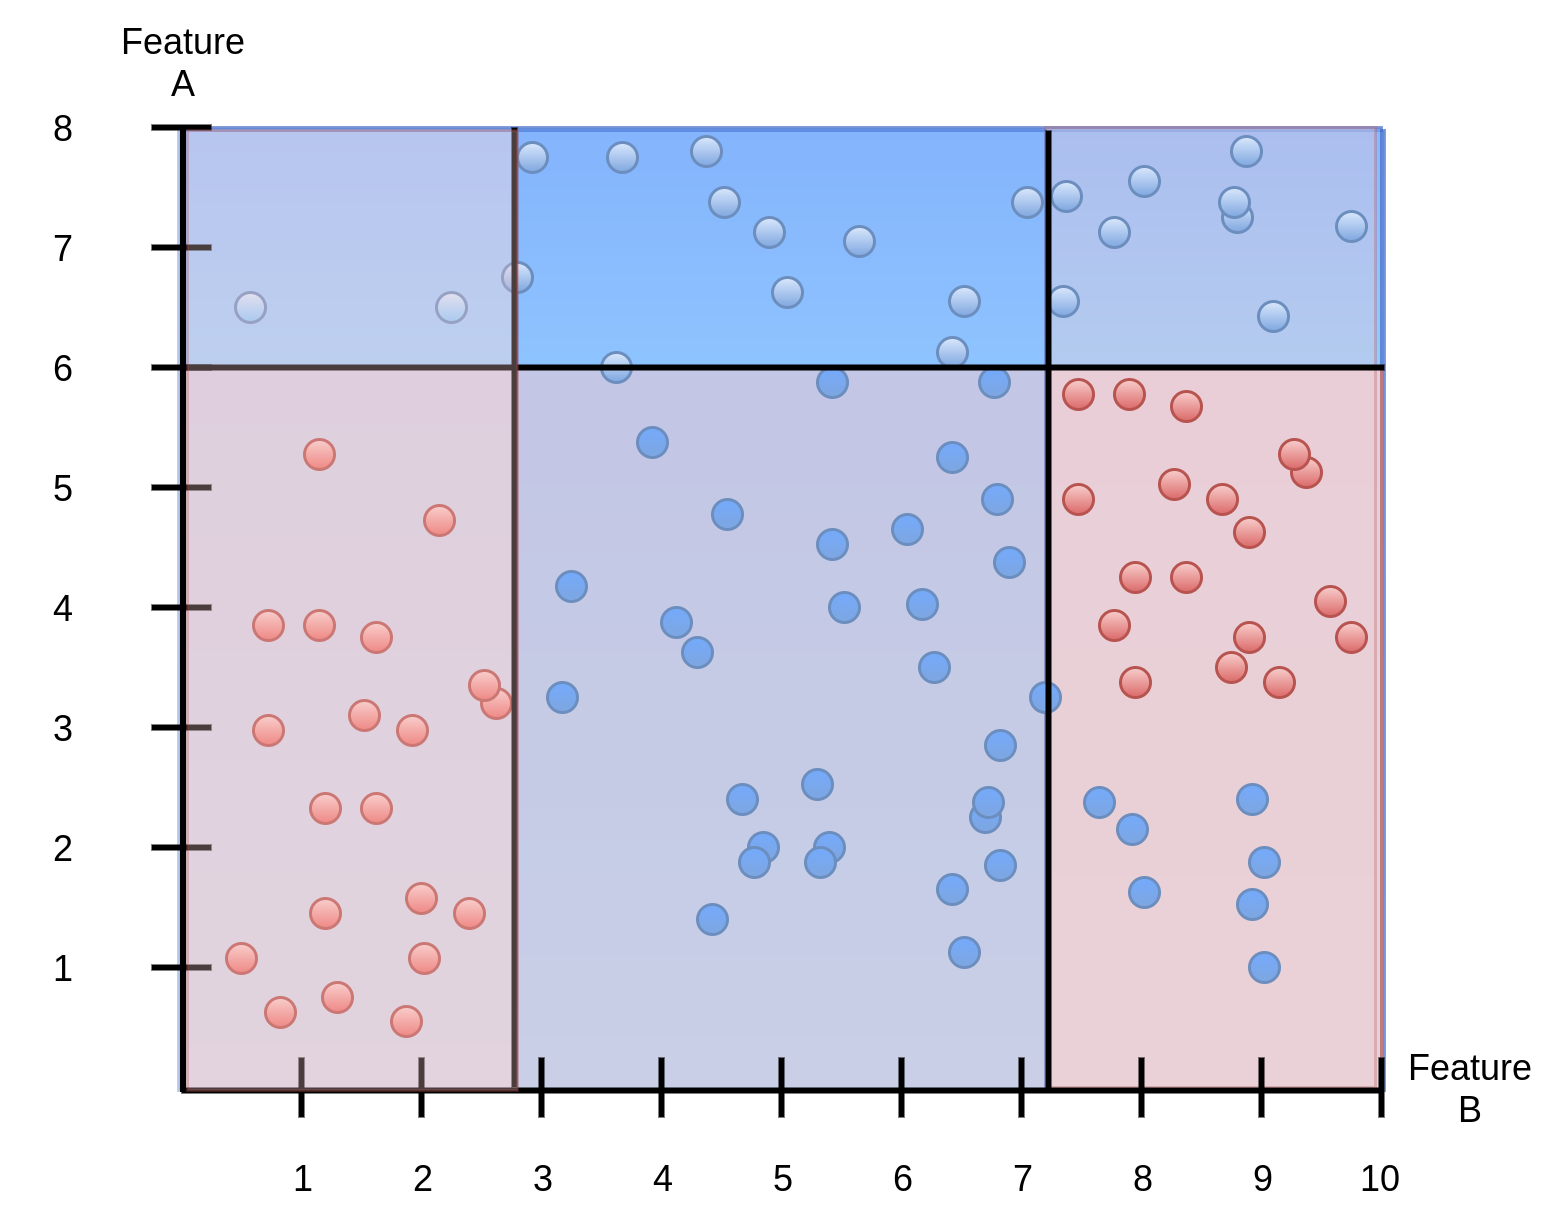
\includegraphics[width=\textwidth]{boosting5}
                    \end{figure} 
                    
                    \par The picture is starting to form. Just with these three weak classifiers, the in-sample error is beginning to swiftly diminish. All the blue points above 6 on the y-axis are correctly classified as blue. The red clusters on either side, as well as the center blue cluster have also found their way to correct classification. In fact, only misclassified points remaining are the blue samples in the lower right. With additional weak classifiers, they too will be captured, as their weight will now be increased.
                    
                    \par Once the algorithm has completed training by either achieving a certain in-sample accuracy or exhausting the number of weak classifiers allowed, a new observation is predicted to be either blue or red depending on whether the area it maps onto is blue or red\footnote{Which corresponds to checking each of the weak classifiers for their answer, adding up their weighted answers and taking the sign.}.
                    
    \newpage

    \section{Methodology}
                    
             \par This section walks through the process by which this project was completed, detailing the work done and the challenges encountered along the way.
             
             \subsection{Research}
             
                 \par As of the writing of this text, TCD has no machine learning options within it's four year curriculum. Consequently, other sources had been sought.
                 
                 \par In preparation for the project, I read "Artificial Intelligence: A Modern Approach"\cite{modernApproach}. Although it is a great introduction to the field, it proved mostly irrelevant to this project\footnote{Gradient descent and a tiny section on neural networks aside.}. 
                 
                 \par It was found that the Massachusetts Institute of Technology make some of their courses available to the public, in particular, their course on artificial intelligence, 6.043\cite{mit}. However, even though over-all superb, I found that both neural networks and kernel functions needed more attention and explanation. The California Institute of Technology machine learning course\cite{caltech} dealt with both of those deficiencies. The California Institute of Technology course also included some very useful background and fundamentals of machine learning. 
                 
                 \par Having worked through and understood all of the above I felt I had a thorough understanding of the techniques used in this project.
                 
             \subsection{Dataset Gathering}
             
                 \par I had decided to apply machine learning to the game of Defence of the Ancients\footnote{DOTA.} 2, having seen some very rudimentary frequency counting already done in the form of a statistics website\cite{dotabuff}.
                 
                 \par I decided to investigate the impact team composition has on match outcome, regardless of any other details about the match. For this, I needed a labelled dataset. It was found that one or two already existed, however, they were useless. The datasets were scarcely documented, making them difficult to use. However, a far more serious detriment to the previous datasets is that DOTA is a volatile game with regards to hero balance and mechanics. New heroes are added, old ones drastically changed. Any sufficiently old dataset no longer reflects the current state of affairs. Thus, a new dataset had to be constructed.
                 
                 \par I had found a blog post by one of the DOTA developers\cite{dotaAPI}, which appeared to be the extent of the official documentation. I already had a steam account and retrieved a key for use within the API. After a few rudimentary queries, I set to developing a wrapper for the API. 
                 
                 \par In development of this I had found an already developed python API for requesting match details\cite{pythonAPI}. After reading the documentation and writing a few test scripts, I wrote a script which uses this API to gather data. I filtered the data by skill, taking only the highly skilled players, and match type, taking only competitive matches, in hopes that highly skilled, competitive matches will be a less noisy dataset with respect to team composition and it's effects.
                 
                 \par There were quite a few obstacles along the way. After the first time of letting the script run overnight, I found the process has crashed, and that the DOTA API was prone to downtime. If the API is down, it will return a null object, which my script will then attempt to parse and crash, losing all data collected thus far. The script was then augmented with error handling.
                 
                 \par On encountering an exception, the error handling wrote the data collected thus far to disk. Unfortunately, the machine used for this work had only a 128GB SSD, and the Ubuntu partition was smaller still. An exception occurred due to the API being down, the script tried to write to disk, then an exception occurred within the error handling and once again data was lost. The Ubuntu partition was then expanded.
                 
                 \par The data gathered was in the form of 10 hero ids, 5 for the Dire team and 5 for the Radiant team, and a binary label indicating a Radiant win or a Dire win. The dataset was thus had 10 dimensions to capture the 10 players' hero choice, as well as a dimension for match outcome.
                 
             \subsection{Machine Learning}
             
                 \par Having done the research, choosing a library to use to the machine learning was simple, as it simply needed to have the tools required. In the end, Scikit-learn\cite{sklearn} had the most accessible documentation, as well as all of the desired functionality\footnote{Tensorflow lacked boosting, and seemed in general far less user-friendly than scikit.}.
                 
                 \subsubsection{Nearest Neighbours}
                     
                     \par I began with nearest neighbours, and consequently, the majority of the learning with respect to Scikit-learn was done here.
                     
                     \par The most naive approach to nearest neighbours was, given a test sample, find the nearest neighbour training sample and predict an identical outcome. This approach gave an accuracy which was worse than simply flipping a coin.
                     
                     \par The next approach was taking several nearest neighbours, averaging their outcome, and predicting based on that. Namely, if 5 nearest neighbours were taken, and 3 of them were a Radiant win, a Radiant win would be predicted. This improved the accuracy slightly, but only barely so. 
                     
                     \par During the averaging of multiple neighbours, I found that the API returned the distance of the neighbours, as well as the neighbours themselves. Consequently, the approach was improved to take a weighted average prediction, as opposed to an unweighted previous attempt. The more similar the match was to the query, the more it's contribution counted towards the prediction. This once again improved the result.
                     
                     \par However, in thinking about the distance, I realized that the current representation of the problem implied a false ordering. A hero with id of 110 is nothing like the hero with id 111, yet if plotted, the distance between them will be small, implying a similarity. This false similarity will then give rise to false nearest neighbours. Hero choice is categorical data, not numerical, and thus required a different representation. 
                     
                     \par Thus began data preprocessing for various methods. The dataset was converted to a one hot encoding\cite{oneHotEncoding}. In this case, take a single player's hero choice. There are currently 113 heroes within the game\cite{dota2Heroes}. A single player's hero choice was a single integer in an array of ten integers. Now that single integer will be converted to an array of 113 elements. Each of those integers will again be an integer\footnote{Although a boolean would suffice.}. All of those 113 elements shall be zero, except for one, at the index of the hero which was chosen. To put it succinctly, in the case that hero with id of 1 was chosen: [1] \(\mapsto\) [0, 1, 0, 0, 0....].
                     
                     \par Converting each of the ten hero choices to one hot encoding leads to 1130 dimensions\footnote{10 heroes times 113.}. Doing this, in addition to taking the weighted average yielded the best results.
                     
                 \subsubsection{Neural Network}
                 
                     \par Scikit-learn provided a simple API to train the neural network, and a default configuration for said network, namely, a neural network with a single hidden layer of 100 neurons. Upon some quick testing however it was found, however, that the default configuration required adjustment of hyper-parameters.
                     
                     \par The machine learning algorithms discussed in the background section are tasked with adjusting the parameters of some model. If we for instance take a simple line, the parameters of that line are it's slope, and it's y-intercept. By adjusting those parameters, we optimize the model to maximize in-sample performance.
                     
                     \par However, there are parameters which are at the discretion of the user, which user-decided parameters influence the optimization of the model parameters. They are so-called hyper-parameters. In the case of the neural network, such parameters are the structure of the neural net, the learning rate\footnote{If applicable.} of gradient descent and so forth.
                     
                     \par I began by manually testing a few configurations of the neural network and noting the performance. After a few of these tests and some research I came across grid search. Grid search is simply the practice of automating the search for hyper-parameters\footnote{Although it could be used for parameter search, such a search would be vastly inferior to the methods discussed in the background section.}. However\foornote{Somewhat amusingly.} there were hyper, or hyper-hyper parameters involved with grid search, namely the parameters which dictated how many and what resources were available to the search. 
                     
                     \par After optimizing the neural net structure by optimizing the grid search, the performance improved. However, as this was being developed, I learned that neural networks are sensitive to feature scaling\cite{skNeuralNet}. Feature scaling, as the name would suggest, involves scaling the training and testing features. An example would be downscaling them all such that all the input features are within the range [-1, +1]. The Scikit library however had a standard scaler.
                     
                     \par Optimal observed performance was achieved after pre-processing the training and testing data by converting to one hot encoding and then applying default suggested scaling as per the documentation in\cite{skNeuralNet}.
                     
                    \subsubsection{Support Vector Machine}
                 
                     \par As with the other models, hyper-parameter estimation was most of what was there to be done with respect to Support Vector Machines. Both the machine\footnote{In the form of the parameter for penalizing margin violation}, and the kernel\footnote{Namely the gamma in the radial basis kernel function.} required optimization.
                     
                     \par A logarithmic grid search was used. This means that the hyper-parameters varied on orders of magnitude\footnote{Powers of 2 in this case}. So a sample parameter would be tested on values of 2, 4, 8, 16 and so forth. This is in accordance to recommendation by the developers of the SVM implementation used in this project\cite{svmGuide}.
                     
                \subsubsection{Boosting}
                    
                    \par By the time boosting was applied, I was quite familiar with the tools at hand and ran into no issues. Using a simple grid search I optimized the key parameter, number of weak classifiers, to yield the best result out of all of the learning methods.
                    
    \section{Implementation}
    
        \par Most of the work went into simply thoroughly understanding the learning methods used in this project. Almost all of the tools required were readily provided by Scikit\cite{sklearn}. Only the data gathering was written from scratch, but even that was aided by a library\cite{pythonAPI}.
        
        \par Upon request, the DOTA 2 server would reply with 100 most recent matches, filtered by specification. However, requests for new data were fired every 5 seconds or so\footnote{In order not to assault the public API with requests.}. As a consequence, every response featured fewer than 100 new matches. In order not to double log already stored match data, a hash table was kept, keeping track of already logged matches.
        
        \par The API server would also frequently go down, resulting in a crash of the data gathering script. The script was then iterated upon to be able to handle server outages.
        
        \par Power outages, however, could not be controlled for. Consequently, another script was written to stitch together various resulting data files, whilst ensuring games were not double-logged.
        
        \par The rest of the implementation was simply becoming familiar with the Scikit-learn API and using the tools it provided, along with the understanding I gained in researching the field, to train the models I had hoped to train.
        
    \section{Results}

                
          
    \printbibliography

\end{document}
